\documentclass[10pt,a4paper]{article}
\usepackage[margin=0.88in]{geometry}
\usepackage{amsmath,amssymb,amsthm,booktabs,array,longtable,xcolor,framed,bm,graphicx}
\usepackage[hidelinks]{hyperref}
\graphicspath{{comp_theory_fig/}}

\theoremstyle{definition}
\newtheorem{defn}{Definition}[section]
\theoremstyle{plain}
\newtheorem{thm}[defn]{Theorem}
\newtheorem{prop}[defn]{Proposition}
\newtheorem{lem}[defn]{Lemma}
\theoremstyle{remark}
\newtheorem{rem}[defn]{Remark}

\definecolor{codeblue}{HTML}{1F4E79}
\definecolor{lightgrey}{HTML}{F4F4F4}

% code-pointer environment: the 20% that maps theory to the deployed files
\newenvironment{codehint}%
  {\par\vspace{2pt}\begin{framed}\noindent\small\textcolor{codeblue}{\textbf{In the code.}}\ }%
  {\end{framed}\vspace{2pt}}

\newcommand{\file}[1]{\textcolor{codeblue}{\texttt{#1}}}
\newcommand{\code}[1]{\texttt{#1}}
\newcommand{\R}{\mathbb{R}}
\newcommand{\E}{\mathbb{E}}
\newcommand{\Lag}{\mathcal{L}}
\newcommand{\Tcheb}{T}
\newcommand{\st}{\mathbf{S}}
\newcommand{\unk}{\mathbf{x}}
\newcommand{\pol}{\bm{\theta}}
\newcommand{\half}{\tfrac{1}{2}}
\DeclareMathOperator*{\argmin}{arg\,min}

\setlength{\parskip}{0.5pt}\setlength{\parindent}{1.1em}
\linespread{0.97}\selectfont
\makeatletter
\renewcommand\section{\@startsection{section}{1}{\z@}%
  {-1.6ex \@plus -.4ex \@minus -.2ex}{0.7ex \@plus.2ex}{\normalfont\large\bfseries}}
\renewcommand\subsection{\@startsection{subsection}{2}{\z@}%
  {-1.1ex\@plus -.3ex \@minus -.2ex}{0.4ex \@plus .2ex}{\normalfont\normalsize\bfseries}}
\setlength{\abovedisplayskip}{3pt}\setlength{\belowdisplayskip}{3pt}
\setlength{\abovedisplayshortskip}{1pt}\setlength{\belowdisplayshortskip}{2pt}
\setlength{\textfloatsep}{6pt}\setlength{\intextsep}{6pt}
\makeatother
\renewcommand{\arraystretch}{1.04}

\title{\vspace{-2.2em}\textbf{Computational Methods for a Global Solution\\of a Two-Country Model with
Occasionally Binding\\Financial Constraints}\\[0.6em]
\large A Theory-First Guide to the Algorithms, and to the Levers that Control Them}
\author{Technical companion to the \textsc{Quantitative\_Model} repository}
\date{5 October 2026}

\begin{document}
\maketitle
\thispagestyle{empty}

\begin{center}
\begin{minipage}{0.88\textwidth}
\small
\noindent\textbf{What this document is.} A self-contained account of the numerical mathematics
behind the two solvers in this repository: a \emph{global Chebyshev--Smolyak projection}
solver for a nonlinear model with an occasionally binding incentive constraint, and a
\emph{sequence-space Jacobian} solver for its linearised sticky-price twin. The emphasis is
roughly four-to-one on theory over implementation: every algorithm is stated as a
mathematical object first, with its convergence properties, its failure modes, and the
parameters (``levers'') that move it. Code is referenced only as a pointer, in marked
boxes, so that a reader can find the deployed counterpart of each construct without the
document becoming a code walkthrough.

\medskip
\noindent\textbf{Who it is for.} Early-stage doctoral students who know what a recursive
competitive equilibrium is, have met value-function iteration and perturbation methods, and
now need to understand what a production global solver actually does --- and, more
importantly, \emph{why each design choice is the one that works}. Prior exposure to
heterogeneous-agent macroeconomics and to financial-accelerator models is assumed; prior
exposure to approximation theory is not.
\end{minipage}
\end{center}
\vspace{0.4em}\setcounter{tocdepth}{1}{\footnotesize\tableofcontents}

%=====================================================================
\vspace{-4pt}\part*{Part I \quad The Computational Problem}
\addcontentsline{toc}{section}{\textbf{Part I\quad The Computational Problem}}
%=====================================================================
\section{What is being solved}

\subsection{The economic object}

The model is a monetary union of two countries, $D$ (small, risky) and $F$ (large, safe).
Each country has a continuum of households facing idiosyncratic income risk and a borrowing
constraint; a representative firm with Cobb--Douglas technology; a capital producer with
convex adjustment costs; a government issuing long-duration perpetuity debt under a fiscal
feedback rule; and --- the mechanism that makes the problem hard --- a
Gertler--Karadi/Bocola financial intermediary whose balance sheet is limited by an
\emph{incentive constraint} that binds only sometimes.

Write the intermediary's problem informally. A banker enters the period with net worth $n$,
chooses a portfolio of assets $A$ (capital, two sovereign bonds, working-capital loans),
funds the gap $A-n$ with deposits, and may abscond with a fraction $\lambda$ of the assets.
Depositors lend only if the franchise value of continuing exceeds the diversion payoff:
\begin{equation}
  \underbrace{\alpha(\st)\,n}_{\text{franchise value}} \;\ge\; \underbrace{\lambda A}_{\text{diversion payoff}},
  \label{eq:IC}
\end{equation}
with multiplier $\mu \ge 0$ and complementary slackness $\mu\,[\alpha n - \lambda A]=0$. When
\eqref{eq:IC} is slack the banker is unconstrained and asset prices satisfy textbook Euler
equations; when it binds, a wedge $\lambda\mu/\E[\Omega]$ opens between the return on
intermediated assets and the deposit rate, and that wedge is the entire transmission channel
from financial distress to real activity in this model.

\subsection{Why this cannot be solved by perturbation alone}

Three features of \eqref{eq:IC} defeat local methods.

\begin{enumerate}
\item \textbf{The constraint is occasionally binding.} The equilibrium conditions are not
differentiable in the state: $\mu(\st) = \max\{\cdot,0\}$ is $C^0$ but not $C^1$ at the
switching boundary. A Taylor expansion around a point is an expansion around one
\emph{regime}; it cannot represent the switch. Worse, as Section \ref{sec:kink} documents,
this economy's ergodic rest point sits \emph{on} the switching boundary, which is precisely
where a smooth approximant is least reliable.

\item \textbf{Risk is priced, and pricing risk is a second-order object.} The mechanism of
interest --- an exogenous rise in the \emph{priced} probability of sovereign default
marks a long bond down, destroys bank equity, tightens \eqref{eq:IC}, raises the lending
spread and contracts output --- lives in the covariance between the stochastic discount
factor and the bond payoff. A first-order perturbation sets that covariance to its
steady-state value by construction. One therefore needs either a higher-order expansion
(which still cannot handle the kink) or a genuinely global method.

\item \textbf{The feared event is large.} The default branch is a $55\%$ write-down on the
whole claim. Nothing local survives a shock of that size: the post-default economy is not a
small deviation from the pre-default one, and the \emph{expectation} taken in today's bond
price must integrate over both branches at their true distance apart.
\end{enumerate}

The response is to solve the model \emph{globally}: to approximate the equilibrium decision
rules as explicit functions on a region of the state space, and to impose the equilibrium
conditions at enough points in that region to pin the approximation down. That is the
subject of Parts II--IV.

\subsection{The functional equation}

Collect the endogenous state in a vector $\st \in \mathcal{S}\subset\R^{d}$ and the
period's unknown allocations in $\unk\in\R^{K}$. A recursive competitive equilibrium is a
collection of \emph{decision rules} $g:\mathcal{S}\times\{0,1\}\to\R^{K}$ --- one set per
discrete regime, here the realised-default indicator $d'\in\{0,1\}$ --- together with a law
of motion $\st' = H(\st,\unk,\epsilon')$, satisfying
\begin{equation}
  \boxed{\;
  \mathcal{F}\big(\st,\,d,\,g(\st,d),\,g(\cdot,\cdot)\big) \;=\; \bm{0}
  \qquad\text{for all } \st\in\mathcal{S},\; d\in\{0,1\}.}
  \label{eq:functional}
\end{equation}
Here $\mathcal{F}$ is a vector of $K$ equilibrium conditions --- Euler equations, market
clearing, first-order conditions, complementarity conditions --- and the third argument
appears \emph{inside an expectation}: evaluating $\mathcal{F}$ at one state requires knowing
$g$ at every state reachable next period. Equation \eqref{eq:functional} is therefore a
\emph{functional} equation: the unknown is a function, and the equation must hold at a
continuum of points.

Two approximations convert \eqref{eq:functional} into something a computer can solve:
\begin{description}
\item[Approximate the function.] Replace $g$ by $\hat g(\cdot\,;\pol)$, a member of a
finite-dimensional family indexed by coefficients $\pol$. Part II is about choosing that
family well.
\item[Approximate ``for all $\st$''.] Impose \eqref{eq:functional} only at a finite set of
\emph{collocation points} $\{\st_i\}_{i=1}^{n}\subset\mathcal{S}$, chosen so that the finite
system has as many equations as unknowns. Part III is about solving the resulting finite
system.
\end{description}

\subsection{Two solvers, one model, different jobs}

The repository carries two independent solvers and they are not substitutes.

\begin{center}
\small
\begin{tabular}{@{}p{0.29\textwidth}p{0.32\textwidth}p{0.32\textwidth}@{}}
\toprule
 & \textbf{Global projection} & \textbf{Sequence-space (SSJ)} \\
\midrule
Mathematical object & recursive decision rules on a region of the state space & impulse-response
Jacobian around a point \\
Nonlinearity & fully nonlinear; the constraint switches & linearised; the constraint's regime
is fixed \\
Unknown & $\pol\in\R^{4600}$ (policy values at nodes) & $\mathbf{U}\in\R^{27T}$ (unknown paths) \\
Solved by & one damped Newton on the whole coefficient vector & one linear solve
$G=-H_U^{-1}H_Z$ \\
Cost & hours & minutes \\
Carries & occasionally binding IC, priced default, two regimes & sticky prices, nominal
deposit contracts, the paper's figures \\
\bottomrule
\end{tabular}
\end{center}

\noindent The two are calibrated differently and their impulse magnitudes are not
comparable. Parts II--VI concern the global solver; Part VII treats the sequence-space
method, whose mathematics is entirely different and worth knowing in its own right.

\begin{codehint}
\file{run.py} is the single entry point and holds the solver settings (grid resolution,
which experiments run); the economics live in \file{calibration/}. The global pipeline is
\code{compute\_global()}/\code{plot\_global()} in \file{run.py}; the linear pipeline is
\file{linear\_ssj/main.py}. The two need different Python interpreters.
\end{codehint}

%=====================================================================
\vspace{-4pt}\part*{Part II \quad Approximating Functions of Many Variables}
\addcontentsline{toc}{section}{\textbf{Part II\quad Approximating Functions of Many Variables}}
%=====================================================================
\section{Chebyshev interpolation in one dimension}
\label{sec:cheb}

Everything in Part II is built from the one-dimensional case, so it pays to understand that
case properly.

\subsection{The question approximation theory actually answers}

The Weierstrass theorem says that any continuous $f$ on $[-1,1]$ is uniformly approximable by
polynomials. It is useless operationally: it does not say which polynomial, and it does not
say how the error falls with degree. The constructive questions are:
\emph{given $m$ evaluations of $f$, where should they be taken, and what is the resulting
error?}

Fix the family: polynomials of degree $\le m-1$, written in the \emph{Chebyshev basis}
\begin{equation}
  \Tcheb_k(u) = \cos\!\big(k\arccos u\big),\qquad u\in[-1,1],\qquad k = 0,1,2,\dots
\end{equation}
These satisfy the three-term recurrence
\begin{equation}
  \Tcheb_0(u)=1,\quad \Tcheb_1(u)=u,\quad
  \Tcheb_{k}(u) = 2u\,\Tcheb_{k-1}(u) - \Tcheb_{k-2}(u),
  \label{eq:recurrence}
\end{equation}
which is how they are evaluated in practice: \eqref{eq:recurrence} is $O(m)$ per point,
backward-stable, and needs no special functions.

\begin{codehint}
\code{chebyshev\_basis\_1d(x, max\_deg)} in \file{global\_projection/solver\_recursive/state\_grid.py}
is exactly \eqref{eq:recurrence}, filling an $(\text{points}) \times (\text{max\_deg}+1)$ matrix
column by column.
\end{codehint}

\subsection{Why node placement is the whole game}

Let $\mathcal{I}_m f$ denote the degree-$(m{-}1)$ polynomial interpolating $f$ at nodes
$u_1<\dots<u_m$. The error splits into a \emph{best-approximation} part and an
\emph{amplification} part:
\begin{equation}
  \|f - \mathcal{I}_m f\|_\infty \;\le\; \big(1+\Lambda_m\big)\,
  \inf_{p\in\mathcal{P}_{m-1}} \|f-p\|_\infty,
  \label{eq:lebesgue}
\end{equation}
where $\Lambda_m = \big\|\sum_{j=1}^m |\ell_j|\big\|_\infty$ is the \emph{Lebesgue constant}
of the node set and $\ell_j$ are the Lagrange basis polynomials. Equation
\eqref{eq:lebesgue} is the key organising fact: the best polynomial may be excellent, but
interpolation at badly chosen nodes amplifies its error by $\Lambda_m$, and
\begin{align}
  \text{equispaced nodes:}&\quad \Lambda_m \sim \frac{2^m}{e\,m\log m} \quad\text{(exponential)},\\
  \text{Chebyshev nodes:}&\quad \Lambda_m \sim \frac{2}{\pi}\log m + O(1) \quad\text{(logarithmic)}.
\end{align}
An exponentially growing amplification factor is what produces the \emph{Runge phenomenon}:
wild oscillation near the endpoints, worsening with degree, even for a perfectly smooth $f$.
Figure \ref{fig:nodes} shows all three facts --- the node families, the resulting degree-14
interpolants of Runge's function $f(u)=1/(1+25u^2)$, and the uniform error against $m$. The
equispaced error \emph{diverges}; the Chebyshev error falls geometrically to machine
precision.

\begin{figure}[t]
\centering
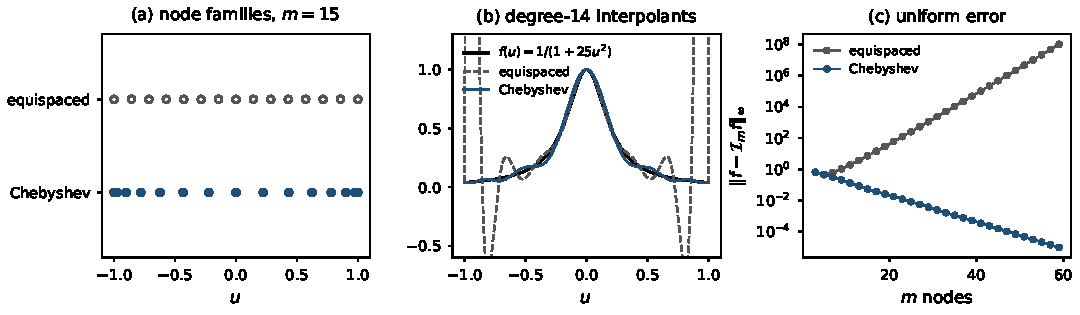
\includegraphics[width=0.82\textwidth]{fig_nodes.pdf}
\caption{\footnotesize Node placement is not a detail. Panel (c) is computed, not schematic: equispaced
interpolation of a smooth function diverges, Chebyshev interpolation of the same function
converges geometrically. The ratio of the two Lebesgue constants at $m=40$ exceeds $10^{9}$.}
\label{fig:nodes}
\end{figure}

\subsection{Which Chebyshev nodes, and why these ones}

Two node families carry the name. The \emph{Chebyshev points of the first kind} (zeros of
$\Tcheb_m$) are $\cos\!\big(\pi(2j{-}1)/2m\big)$; the \emph{points of the second kind}, also
called Chebyshev--Lobatto or Chebyshev \emph{extrema}, are
\begin{equation}
  u_j^{(m)} = -\cos\!\Big(\frac{\pi (j-1)}{m-1}\Big),\qquad j=1,\dots,m.
  \label{eq:extrema}
\end{equation}
Both have logarithmic Lebesgue constants. The solver uses \eqref{eq:extrema}, for a reason
that becomes decisive in Section \ref{sec:smolyak}: the extrema are \emph{nested}. Taking
$m_i = 2^{\,i-1}+1$ points at ``level'' $i$ gives
\begin{equation}
  \mathcal{U}_1 = \{0\} \subset \mathcal{U}_2 = \{-1,0,1\} \subset \mathcal{U}_3 =
  \{-1,-\tfrac{\sqrt2}{2},0,\tfrac{\sqrt2}{2},1\}\subset \cdots
\end{equation}
so that every node of a coarse level survives into every finer level. Nesting is what makes
the sparse-grid construction economical, and it is also what makes \emph{refinement a warm
start}: a solution computed on level $i$ is exactly reusable at level $i{+}1$.

\begin{codehint}
\code{\_level\_points(i)} builds $\mathcal{U}_i$; \code{\_new\_points(i)} returns
$\mathcal{U}_i\setminus\mathcal{U}_{i-1}$, which for $i\ge 3$ is just the odd-indexed
entries (\code{[1::2]}) --- a one-line consequence of nesting.
\end{codehint}

\subsection{Error bounds: the smooth case and the kinked case}

Two regimes of convergence matter here, and the model lives in both.

\begin{thm}[Geometric convergence for analytic functions]
\label{thm:geom}
If $f$ extends analytically to the Bernstein ellipse $E_\rho$ with foci $\pm 1$ and
semi-axis sum $\rho>1$, and $|f|\le M$ on $E_\rho$, then
\begin{equation}
  \|f-\mathcal{I}_m f\|_\infty \;\le\; \frac{4M}{\rho-1}\,\rho^{-(m-1)}.
\end{equation}
\end{thm}
\noindent The error falls \emph{geometrically} in the number of nodes, at a rate set by how
far $f$'s nearest singularity sits from $[-1,1]$. This is the regime the solver wants to be
in, and it explains the shape of Figure \ref{fig:nodes}(c).

\begin{thm}[Algebraic convergence for finitely differentiable functions]
If $f\in C^{k}[-1,1]$ then $\|f-\mathcal{I}_m f\|_\infty = O(m^{-k}\log m)$. For $f\in C^0$
with a single interior kink --- the case $\mu=\max\{\cdot,0\}$ --- the rate is $O(m^{-1})$
and the error does not decay \emph{uniformly}: it concentrates in a shrinking neighbourhood
of the kink, where it is $O(1)$ in a relative sense. This is the \emph{Gibbs phenomenon}.
\end{thm}

Figure \ref{fig:kink} panels (a) and (b) show this directly for $\max(u,0)$. Note the
qualitative behaviour: the overshoot does not vanish as $m$ grows, it merely narrows and
migrates toward the kink. \emph{Refinement does not cure a Gibbs phenomenon; it relocates
it.} Section \ref{sec:kink} shows what this costs the model, and what the honest response is.

\begin{figure}[t]
\centering
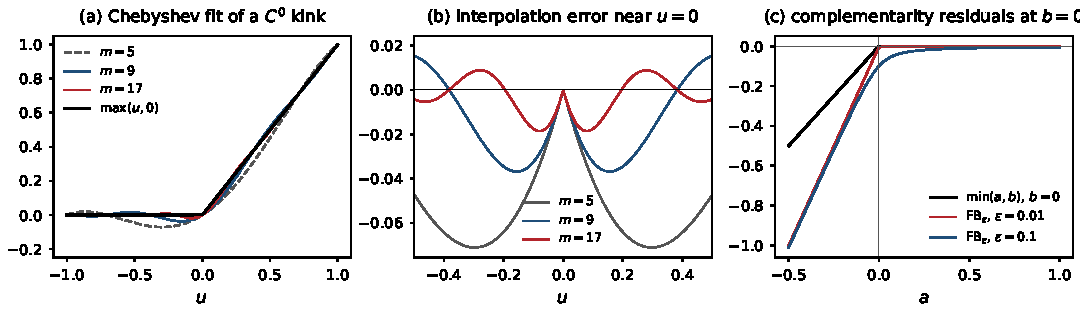
\includegraphics[width=0.82\textwidth]{fig_kink.pdf}
\caption{\footnotesize Nonsmoothness, computed. (a) Chebyshev interpolants of $\max(u,0)$ at three
resolutions: the fit returns strictly positive values where the truth is exactly zero, and
negative values just left of the kink. (b) The error narrows but does not shrink in
amplitude --- a Gibbs phenomenon. (c) Two ways of writing complementarity: $\min(a,b)$ has
\emph{zero slope} in $a$ whenever $b<a$, whereas the smoothed Fischer--Burmeister function
retains slope in both arguments (Section \ref{sec:complementarity}).}
\label{fig:kink}
\end{figure}

\subsection{Collocation versus regression, and why squareness matters}

Given $n$ basis functions and $n$ nodes, interpolation solves the square linear system
\begin{equation}
  \Phi\,\bm{c} = \bm{y},\qquad \Phi_{ij} = \phi_j(u_i),
  \label{eq:collocation}
\end{equation}
and the resulting $\hat f = \sum_j c_j\phi_j$ reproduces $f$ \emph{exactly at the nodes}.
With more nodes than basis functions one would instead run a least-squares regression, which
does not. The distinction is not cosmetic in this application. The global solver treats
\emph{the policy values at the nodes} as its unknowns and reads the continuation value off
the fitted interpolant; if the interpolant did not reproduce its own nodes, the ``value at a
node'' would not be well-defined and the Newton system would be inconsistent with its own
parameterisation. Squareness is thus a structural requirement, not an efficiency choice.

One practical consequence: $\Phi$ is fixed once the grid is built, so it is factorised once
(an $LU$) and every subsequent fit is a triangular solve.

\begin{codehint}
\code{SmolyakGrid.\_\_init\_\_} builds $\Phi$ and stores \code{lu\_factor(\_Phi)};
\code{fit()} is one \code{lu\_solve}. A separate \code{fit\_weighted()} offers masked
ridge-regularised least squares --- deliberately \emph{not} the default, because it breaks
nodal exactness (see the comment in \code{\_install\_guess}).
\end{codehint}

\section{The curse of dimensionality and the Smolyak construction}
\label{sec:smolyak}

\subsection{Why tensor products are hopeless at $d=12$}

The obvious extension of \S\ref{sec:cheb} to $d$ dimensions is the tensor product: take $m$
nodes per dimension, use all $m^d$ combinations, and all $m^d$ product basis functions
$\phi_{\bm{k}}(\bm{u}) = \prod_{j} \Tcheb_{k_j}(u_j)$. The approximation inherits
one-dimensional accuracy in every direction. It also inherits an exponential cost: at the
model's $d=12$ with a modest $m=5$,
\begin{equation}
  m^d = 5^{12} \approx 2.44\times 10^{8}\ \text{points}.
\end{equation}
Each point requires an evaluation of the full period map including multi-branch quadrature.
This is not a tractability-at-the-margin problem; it is off by eight orders of magnitude.

\subsection{The telescoping-difference idea}

Smolyak's construction rests on one observation: most of the tensor-product basis is paying
for \emph{high-order interaction terms} that a smooth function does not need. A function that
is quadratic in each variable separately and has mild pairwise interaction does not require
the degree-$(4,4,4,\dots,4)$ cross terms that the tensor grid buys.

Formalise it. Let $\mathcal{I}^{(i)}$ be the one-dimensional interpolation operator at level
$i$ (using $\mathcal{U}_i$), and define the \emph{difference operator}
\begin{equation}
  \Delta^{(i)} \;=\; \mathcal{I}^{(i)} - \mathcal{I}^{(i-1)},\qquad \mathcal{I}^{(0)} \equiv 0 .
\end{equation}
Then $\mathcal{I}^{(i)} = \sum_{\iota\le i}\Delta^{(\iota)}$ telescopes, and the full
$d$-dimensional tensor operator at level $i$ in every dimension is
\begin{equation}
  \mathcal{I}^{(i)}\otimes\cdots\otimes\mathcal{I}^{(i)}
  = \sum_{\bm{\iota}\,:\,\iota_j\le i\;\forall j} \Delta^{(\iota_1)}\otimes\cdots\otimes\Delta^{(\iota_d)} .
\end{equation}
The sum runs over a $d$-dimensional \emph{cube} of multi-indices. Smolyak's operator keeps
only a \emph{simplex} of them:
\begin{equation}
  \boxed{\;\mathcal{A}_{\mu,d} \;=\; \sum_{\bm{\iota}\,:\,\sum_j (\iota_j-1)\,\le\,\mu}
  \Delta^{(\iota_1)}\otimes\cdots\otimes\Delta^{(\iota_d)} .}
  \label{eq:smolyak}
\end{equation}
The parameter $\mu$ is a \emph{total-level budget}: a term is admitted if the levels it uses,
summed across dimensions, do not exceed $\mu$ above the baseline. High resolution in one
dimension is affordable; high resolution in all dimensions simultaneously is not. The
discarded terms are exactly the high-order interactions.

\begin{prop}[Point count]
\label{prop:count}
With nested node sets, the Smolyak grid is $\mathcal{H}_{\mu,d} =
\bigcup_{\bm{\iota}} \big(\mathcal{U}^{\mathrm{new}}_{\iota_1}\times\cdots\times
\mathcal{U}^{\mathrm{new}}_{\iota_d}\big)$ where $\mathcal{U}^{\mathrm{new}}_{i} =
\mathcal{U}_i\setminus\mathcal{U}_{i-1}$. For $\mu=1$ the count is $1+2d$ --- the centre plus
two endpoints per dimension. For $\mu=2$ it grows as $O(d^2)$, and in general
$|\mathcal{H}_{\mu,d}| = O\!\big(d^{\mu}\big)$: \emph{polynomial in dimension at fixed
budget}, against the tensor grid's exponential.
\end{prop}

\noindent At $d=12$: $\mu=1$ gives $25$ points, $\mu=2$ gives $313$. The problem has gone
from $2.4\times 10^8$ to a few hundred. This is the single most important fact in the
document.

\begin{figure}[t]
\centering
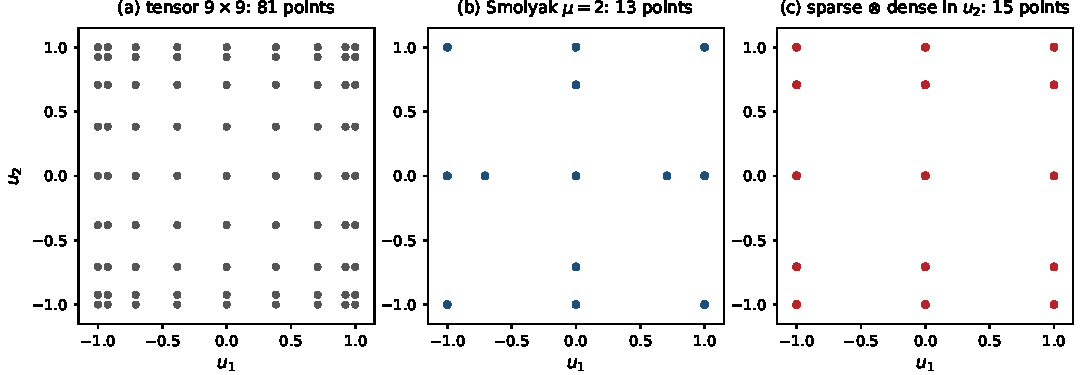
\includegraphics[width=0.82\textwidth]{fig_smolyak.pdf}
\caption{\footnotesize Grid geometry in two dimensions, drawn by the repository's own grid constructor.
(a) The tensor product is dense everywhere. (b) The Smolyak grid at $\mu=2$ keeps the axes
and the coarse interactions, dropping the high-order corners. (c) The construction actually
shipped: a sparse factor over all dimensions but one, tensored with a \emph{dense} factor in
the dimension that carries curvature --- here $u_2$ stands for the sovereign-risk state $s$.}
\label{fig:smolyak}
\end{figure}

\subsection{The square ``new points, new degrees'' form}

Written as \eqref{eq:smolyak}, the Smolyak operator is a signed combination of tensor
interpolants, and implementing it that way means carrying combinatorial coefficients and
re-evaluating overlapping terms. The implementation here uses the equivalent
\emph{Krueger--Kübler} form, which is cleaner and has a property worth naming.

The idea: pair each \emph{new point set} $\mathcal{U}^{\mathrm{new}}_i$ with a matching set of
\emph{new Chebyshev degrees} $\mathcal{D}^{\mathrm{new}}_i$, constructed so that
$|\mathcal{D}^{\mathrm{new}}_i| = |\mathcal{U}^{\mathrm{new}}_i|$:
\begin{equation}
  \mathcal{D}^{\mathrm{new}}_1=\{0\},\quad
  \mathcal{D}^{\mathrm{new}}_2=\{1,2\},\quad
  \mathcal{D}^{\mathrm{new}}_i = \{2^{i-2}+1,\dots,2^{i-1}\}\ (i\ge 3).
\end{equation}
Running the \emph{same} multi-index set $\{\bm{\iota}:\sum_j(\iota_j-1)\le\mu\}$ over degrees
instead of points yields exactly as many basis functions as nodes. The interpolation matrix
$\Phi$ is therefore square, the collocation system \eqref{eq:collocation} is a plain linear
solve, and the interpolant is exact at every node --- the property \S\ref{sec:cheb} argued is
structural.

\begin{prop}[Polynomial exactness]
$\mathcal{A}_{\mu,d}$ reproduces exactly every polynomial in the span of
$\{\prod_j \Tcheb_{k_j} : \bm{k}\in \mathcal{D}_{\mu,d}\}$. At $\mu=1$ that span contains
all constants, all linear terms, and the pure quadratics $u_j^2$ --- but \emph{no} cross
terms $u_ju_k$. At $\mu=2$ it contains all quadratic cross terms.
\end{prop}

\noindent This proposition is the practical guide to choosing $\mu$: ask which interactions
the economics requires. If the only strongly curved object is a function of one state, $\mu=1$
plus refinement in that state suffices. If two states interact nonlinearly, $\mu\ge2$ is not
optional.

\begin{codehint}
\code{\_multi\_indices(d, mu, mu\_vec)} enumerates the simplex depth-first;
\code{\_new\_degrees(i)} is the degree set above; \code{\_sparse\_nodes} takes the union of
tensor products of new-point sets and records the matching degrees. The exactness claim is
regression-tested in \file{Claude files/global\_projection/tests/test\_state\_grid.py}. An
independent check: fitting $1+u_1u_9+u_9^2$ on the shipped grid and evaluating at $200$
random interior points reproduces it to $8.9\times10^{-16}$.
\end{codehint}

\subsection{Anisotropy: per-dimension budgets}

Nothing forces the budget to be isotropic. Replacing the constraint set by
\begin{equation}
  \Big\{\bm{\iota} : \textstyle\sum_j (\iota_j-1) \le \mu \ \text{ and }\ \iota_j - 1 \le \mu_j\ \forall j\Big\}
\end{equation}
caps the resolution dimension by dimension. This is the right instrument when the state
vector is heterogeneous in curvature, which it invariably is: in this model the two capital
stocks are nearly linear in their own arguments, while the risk state $s$ drives a logistic
default probability.

\subsection{The refinement that is actually shipped: sparse $\otimes$ dense}

Anisotropic budgets have a defect. Because the constraint $\sum_j(\iota_j-1)\le\mu$ is
\emph{global}, raising one dimension's cap to reach degree 4 in that dimension requires
raising $\mu$, which then admits high-level terms in \emph{every other} dimension too. On the
$10$-state box, asking for level 2 in the risk dimension alone costs $165$ points; the
isotropic $\mu=2$ grid costs $221$.

The alternative is to make the grid a \emph{Cartesian product of two interpolation
operators}:
\begin{equation}
  \boxed{\;\mathcal{A} \;=\; \mathcal{A}_{\mu,\,d-1}^{\,(\text{all dims but } r)}
  \;\otimes\; \mathcal{I}^{\,m}_{(r)} \;}
  \label{eq:refine}
\end{equation}
where $\mathcal{I}^{m}_{(r)}$ is a \emph{dense} $m$-node Chebyshev interpolant in the single
dimension $r$. Both factors are square interpolation operators, so the product is square and
exact at its nodes --- the structural property survives. What one buys is degree $m-1$ in
dimension $r$ \emph{and full interaction} between that dimension and the entire sparse basis,
at a cost of $|\mathcal{H}_{\mu,d-1}|\times m$ points.

The measured payoff on this model's curvature profile (Figure \ref{fig:convergence}) is
large. Against the isotropic $\mu=2$ grid at $221$ points and relative RMS error
$3.9\times10^{-2}$, the product grid at $m=9$ achieves $1.1\times10^{-3}$ --- about $36$
times more accurate --- using $171$ points, i.e.\ \emph{fewer}. The reason is specific and
instructive: the curvature being resolved is the logistic $p^d(s) = (1+e^{-s})^{-1}$, which a
$\mu=1$ quadratic misfits badly (reading $3.30\%$ where the truth is $1.98\%$ at the headline
shock), and dimension $r=s$ is exactly where the extra degrees go.

\begin{figure}[t]
\centering
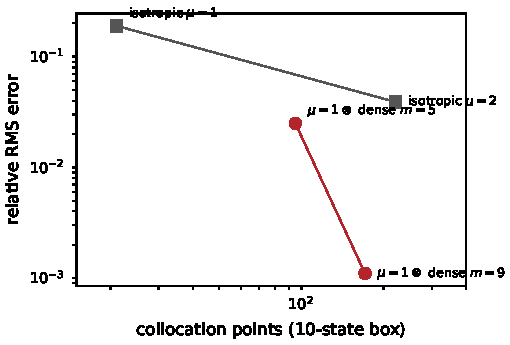
\includegraphics[width=0.62\textwidth]{fig_convergence.pdf}
\caption{\footnotesize Measured relative RMS error against point count, on a test function matching this
model's curvature profile (near-linear in the wealth states, logistic in $s$, with one
interaction). The product construction \eqref{eq:refine} dominates: it is more accurate than
the isotropic $\mu=2$ grid at fewer points, because its extra degrees are spent where the
curvature is.}
\label{fig:convergence}
\end{figure}

\begin{codehint}
\code{SmolyakGrid(..., refine=(dim, m))} implements \eqref{eq:refine} via
\code{\_tensor\_refine}. The shipped setting is \code{S\_REFINE = 5} in \file{run.py}
($115$ points on the $12$-state box); \code{S\_REFINE = 9} is the reference resolution
($207$ points) and the solve ladder walks $5\to9$. Confirmed convergence at $5$: moving to
$9$ shifts the impact output response by $1.6\%$--$3.4\%$ of itself, well inside the
reported identification bracket, and every other headline number moves only in the third
digit.
\end{codehint}

\section{Domain geometry: where the approximation lives}
\label{sec:box}

A global method is global only on a \emph{region}. Choosing that region is a modelling
decision with real consequences, and it is governed by three considerations: coverage,
invariance, and coordinates.

\subsection{The affine map and the coverage question}

The grid is constructed on $[-1,1]^d$ and mapped affinely onto a box
$\prod_j[\underline{S}_j,\overline{S}_j]$:
\begin{equation}
  \bm{u} = 2\,\frac{\st-\underline{\st}}{\overline{\st}-\underline{\st}} - \bm{1},
  \qquad
  \st = \underline{\st} + \half(\bm{u}+\bm{1})\odot(\overline{\st}-\underline{\st}).
\end{equation}
The box must be wide enough that the model's ergodic set lies inside it (otherwise the solver
is extrapolating, and polynomial extrapolation is catastrophic), and narrow enough that the
approximation is not spending its degrees of freedom on states the model never visits.

For a stochastic state the right unit is \emph{coverage in unconditional standard
deviations}, not an absolute width. If $s_t$ is an AR(1) with persistence $\rho_s$ and
innovation standard deviation $\sigma_s$, its unconditional standard deviation is
$\sigma_s/\sqrt{1-\rho_s^2}$, and the box is set to $s^\star \pm \kappa\,
\sigma_s/\sqrt{1-\rho_s^2}$ with $\kappa$ the coverage. Stating the lever this way makes it
invariant to recalibration of $\sigma_s$; an absolute half-width silently changes coverage
whenever $\sigma_s$ moves.

\begin{rem}[A cautionary measurement]
There is a documented episode in which an absolute half-width, chosen when $\sigma_s$ was
$2.4$ times its eventual value, left the box only $1.4$--$2.3$ \emph{conditional} standard
deviations wide. The consequence was not a mild loss of accuracy: because simulated states
are projected back into the box, the clipping mean-reverted $s$ harder than $\rho_s$ did,
cutting the \emph{effective} persistence from $0.95$ to $0.80$ and removing roughly $62\%$ of
the long bond's mark-to-market repricing --- the paper's entire mechanism. A box is part of
the model, not part of the plumbing.
\end{rem}

\subsection{One-step invariance and the non-normality obstruction}

Ideally the box is \emph{forward invariant}: states reachable in one step from inside the box
remain inside. Linearise the law of motion for a sub-block of states around the steady state,
$\st'-\st^{ss} \approx J(\st-\st^{ss})$. A box with half-widths $\bm{b}$ is one-step invariant
if
\begin{equation}
  |J|\,\bm{b} \;\le\; \bm{b} \qquad\text{componentwise},
  \label{eq:invariance}
\end{equation}
where $|J|$ is the entrywise absolute value. By Perron--Frobenius, \eqref{eq:invariance} has a
positive solution $\bm{b}$ if and only if the spectral radius $\rho(|J|)\le 1$. Crucially
$\rho(|J|)$ is \emph{not} $\rho(J)$: for a non-normal $J$ they can differ a great deal.

This model supplies a textbook example. The measured Jacobian of the two banks' gross deposit
obligations $(P_D,P_F)$ at the steady state is
\begin{equation}
  J = \begin{pmatrix} 1.076 & -0.310\\ 2.016 & -1.252\end{pmatrix},
  \qquad \text{eigenvalues } 0.766,\,-0.942,
  \qquad \rho(|J|) = 1.96 .
\end{equation}
The dynamics are \emph{stable} ($\rho(J)<1$) and yet \emph{no axis-aligned box centred on the
steady state is one-step invariant, at any bandwidth}, because $\rho(|J|)>1$. The cause is
non-normality: the singular values are $2.61$ and $0.28$, so the map stretches strongly in one
direction while contracting in another, and an axis-aligned box cannot align with either.

\subsection{Rotation: collocating on the eigenbasis}

The repair is to draw the box in coordinates where $J$ is diagonal. Let $J = V\Lambda V^{-1}$
and collocate on $\bm{z} = V^{-1}(\st - \st^{c})$. In those coordinates the map acts
component-wise with $|\lambda_j|<1$, so \emph{every} box is invariant. The grid class supports
this by carrying a general invertible $\mathrm{rot}$ and centre, converting on the way in and
out, so that every public method still speaks natural coordinates.

Converting a box specification between coordinate systems requires care. A $\bm{z}$-box with
half-widths $\bm{b}$ reaches natural half-widths $|V|\,\bm{b}$, so to reach prescribed natural
half-widths $\bm{t}$ one solves $|V|\bm{b} = \bm{t}$ --- and falls back to the superset
$\bm{b} = |V|\bm{t}$ if that has no positive solution.

\begin{rem}[Theory wins, measurement decides]
The rotation is \emph{right in theory} and \emph{measures worse}, so it ships switched off. A
rotated box is a parallelogram in natural coordinates, and its corners reach combinations of
the two deposit obligations at which the period map has no solution. The invariance gained is
worth less than the feasibility lost. This is a recurring pattern in global solution work and
worth internalising early: the correct geometric argument tells you what to try, not what to
keep.
\end{rem}

\subsection{Shear: coordinates on the reachable set}

A second, subtler coordinate problem arises when two states are linked by an \emph{accounting
identity} rather than by dynamics. The central bank's backstop in this model adds two states:
its bond holdings $M$ and its gross obligation $O$ to the banks. A purchase moves bank
holdings $b_{DD}$ and $M$ one-for-one and books $O \approx R\,Q\,M$. The three are therefore
tied, and an axis-aligned box in $(b_{DD}, M, O)$ contains nodes that \emph{no purchase can
reach}: bonds sold with nothing owed, a claim owed with nothing held.

Collocating at unreachable nodes is not a harmless waste. The fitted rule must interpolate
through those nodes, and the measured consequence was a \emph{non-monotone} price response to
a forced purchase ($-0.5\%$ at one size, $+0.3\%$ at another) and a fourfold move in the
constraint multiplier. The repair is a \emph{shear} --- a unit-determinant change of
coordinates putting the box on the reachable directions:
\begin{equation}
  z_{b} = b_{DD} + M, \qquad z_{O} = O - \rho\,M, \qquad \rho \equiv (1+r^{dep})\,Q^{ss},
\end{equation}
i.e.\ ``what the bank would hold absent the backstop'' and ``the claim net of its
steady-state value''. Because both new states are zero at the steady state and the shear is
unit-triangular, the $M=O=0$ slice is untouched: every node of the smaller grid remains a node
of the larger one, so the backstop-off model \emph{nests} the no-backstop solution exactly
rather than approximately (measured agreement of the rules: $5.5\times10^{-10}$).

\begin{codehint}
\code{build\_state\_box} composes the optional $P$-rotation with the backstop shear (they
touch disjoint rows) and hands the product to \code{SmolyakGrid(rot=...)}.
\code{\_rotate\_box} performs the half-width conversion; \code{outside()} reports per-state
box violation as a fraction of width, which is the invariance diagnostic of
\S\ref{sec:accuracy}. Nesting is asserted in
\file{Claude files/global\_projection/tests/test\_recursive\_nesting.py}.
\end{codehint}

%=====================================================================
\vspace{-4pt}\part*{Part III \quad Solving the Discretised System}
\addcontentsline{toc}{section}{\textbf{Part III\quad Solving the Discretised System}}
%=====================================================================
\section{Two paradigms: iterate, or solve}
\label{sec:paradigms}

With the function space fixed, \eqref{eq:functional} becomes a finite system. There are two
fundamentally different ways to attack it, and the difference matters far more than it looks.

\subsection{Time iteration as a fixed-point problem}

The traditional approach constructs an operator. Fix a guess $\hat g^{(k)}$ for the decision
rules. At each collocation point $\st_i$, treat $\hat g^{(k)}$ as the \emph{frozen
continuation} --- the function used to evaluate next period inside the expectation --- and
solve the $K$ period-$t$ equilibrium conditions for the $K$ unknowns at that point:
\begin{equation}
  \unk_i^{\,\text{new}} : \quad \mathcal{F}\big(\st_i,\,d,\,\unk_i^{\,\text{new}},\,\hat g^{(k)}\big) = \bm 0 .
  \label{eq:timeiter}
\end{equation}
Then fit a new interpolant through $\{\unk_i^{\text{new}}\}$, optionally damp, and repeat:
\begin{equation}
  \hat g^{(k+1)} = (1-\omega)\,\hat g^{(k)} + \omega\,\mathcal{T}\!\big[\hat g^{(k)}\big].
\end{equation}
This is attractive. Each pointwise solve is small ($K=14$ unknowns here, not $4600$), the
points are independent, and if $\mathcal{T}$ is a contraction the iteration converges globally
from a crude start. It is the workhorse of the literature.

\subsection{The contraction rate is the problem}

Suppose $\mathcal{T}$ is a contraction with modulus $\rho$. Convergence is \emph{linear}:
$\|\hat g^{(k)} - g\| \lesssim \rho^{k}$. Two consequences follow, and both bite here.

\begin{prop}[Level error implied by a change-based stopping rule]
\label{prop:stall}
If the iteration converges at rate $\rho$ and one stops when the \emph{change}
$\|\hat g^{(k+1)}-\hat g^{(k)}\|$ falls below $\tau$, the remaining \emph{level} error is
\begin{equation}
  \|\hat g^{(k)} - g\| \;\approx\; \frac{\tau}{1-\rho}.
\end{equation}
\end{prop}
\noindent At $\rho = 0.99$, a stopping tolerance of $\tau=10^{-6}$ admits a level error of
$10^{-4}$. That is not a tight solution, and nothing in the diagnostics reveals it.

Now the measured $\rho$ for this model. The binding mode is the banker's franchise-value
recursion
\begin{equation}
  \alpha = \frac{\E[\Omega]\,R}{1-\mu},\qquad \Omega = \beta\big[f + (1-f)\,\alpha'\big],
\end{equation}
whose slope in $\alpha'$ is $\beta(1-f)R/(1-\mu) \approx 0.96$. With damping $\omega=0.25$
the effective per-sweep modulus is $1-\omega(1-0.96) \approx 0.990$, i.e.\ roughly $235$
sweeps per decade of rule change. The symptom observed in practice is diagnostic and should
be recognised: runs reported $\max|\mathcal{F}| = 10^{-14}$ \emph{and} ``rule-change tolerance
not reached'' simultaneously. Every collocation point was clearing \emph{perfectly against a
continuation that was still moving}. The residual, the natural object to monitor, was
silent about the error.

\subsection{Simultaneous collocation: make the policy values the unknowns}

The alternative abandons the operator view. Define the unknown vector to be the policy
\emph{values at every node, in every regime}:
\begin{equation}
  \pol \;=\; \Big(\,\hat x_{k}(\st_i,d)\,\Big)_{k=1,\dots,R;\ d=0,1;\ i=1,\dots,n} \;\in\; \R^{R\cdot 2\cdot n},
\end{equation}
and define a single global residual map $F : \R^{R\cdot2\cdot n}\to\R^{N_{\mathrm{res}}\cdot2\cdot n}$ by:
\begin{quote}
\emph{(i)} fit the Chebyshev coefficients to $\pol$; \emph{(ii)} at every $(\st_i,d)$, walk
the period map using \emph{that} interpolant as the continuation; \emph{(iii)} stack the
equilibrium residuals.
\end{quote}
Then solve $F(\pol)=\bm 0$ by Newton's method. There is no inner root-find and no frozen
continuation: \emph{the continuation is always the current guess}. The fixed point is not
approached at some rate --- the residual itself is driven to its arithmetic floor, and there
is no contraction modulus for error to leak through.

The two paradigms are compared below.
\begin{center}\small
\begin{tabular}{@{}p{0.2\textwidth}p{0.36\textwidth}p{0.36\textwidth}@{}}
\toprule
 & \textbf{Time iteration} & \textbf{Simultaneous collocation} \\
\midrule
Unknowns per solve & $K=14$, repeated $2n$ times & $R\cdot2n = 4600$, once \\
Continuation & previous iterate (frozen) & the current guess (self-consistent) \\
Convergence & linear at $\rho\approx 0.99$ & quadratic in a neighbourhood \\
Stopping on & rule change (admits $\tau/(1{-}\rho)$) & the residual itself \\
Cost per step & $2n$ small root-finds & one dense Jacobian: $4601$ residual evaluations \\
Role here & \textbf{warm start only} & \textbf{the solver} \\
\bottomrule
\end{tabular}
\end{center}

\subsection{The subtle part: self-reference and the identity residuals}

Making \emph{everything} an unknown requires care about objects that the pointwise method
used to \emph{read off} a recursion rather than solve for. In this model six such objects
exist: the two banker franchise values $\alpha_D,\alpha_F$, the two consumptions
$C_D,C_F$, and the two working-capital rates $r^{wc}_D, r^{wc}_F$. In time iteration these are
computed from the frozen continuation, stored, and refitted --- which is exactly the knot
Proposition \ref{prop:stall} describes.

Under simultaneous collocation they become unknowns with their own residual. The device is
to impose consistency between the \emph{guessed} value and the \emph{implied} value:
\begin{equation}
  \boxed{\;r_k \;=\; \mathcal{T}_{\!k}\big(\text{guess}_k\big) - \mathcal{T}_{\!k}\big(\text{implied}_k\big)
  \;=\; \log\frac{\text{guess}_k}{\text{implied}_k}\;}
  \label{eq:identity}
\end{equation}
where $\mathcal{T}_k$ is whatever transform the rule is fitted in (log level, or log gross
rate; see \S\ref{sec:transforms}). The logarithm is not cosmetic: it makes the residual
scale-free and dimensionally comparable across objects of very different magnitudes.

The reason this closes the knot exactly is worth stating, because it is the link back to
\S\ref{sec:cheb}: \emph{square collocation interpolates its own nodes}. When the period map
asks for $\alpha$ at the current state and that state \emph{is} a collocation node,
evaluating the fitted interpolant returns the guess exactly. There is no interpolation error
at the node to contaminate \eqref{eq:identity}, and the solved object is a genuine recursive
equilibrium rather than a fixed point of a damped map.

Counting for this model: $14$ market-clearing/Euler/policy residuals from the period map,
plus $6$ identity residuals, for $N_{\mathrm{res}}=20$ per (point, regime) --- matching
$R=20$ stored rules, so the system is square.

\begin{codehint}
\file{collocation.py} is the solver. \code{make\_residual} builds $F(\pol)$ and is the image
of Bocola's \code{residual\_model.m}; \code{pack}/\code{unpack} define the stacking
convention (rule-major, then regime, then point); \code{point\_residuals} in
\file{point\_map.py} is the per-point period map and is \emph{unchanged} between the two
paradigms --- only who calls it and what counts as an unknown differs. The $\log$ in
\eqref{eq:identity} is \code{to\_fit(k, guess) - to\_fit(k, out[k])}.
\end{codehint}

\section{The Newton solver}
\label{sec:newton}

\subsection{Damped Newton with a finite-difference Jacobian}

The iteration is
\begin{equation}
  \pol^{(k+1)} = \pol^{(k)} - c\,\big[J(\pol^{(k)})\big]^{-1} F(\pol^{(k)}),
  \qquad J_{ij} = \frac{\partial F_i}{\partial \theta_j},
  \label{eq:newton}
\end{equation}
with damping $c\in(0,1]$. The Jacobian is built by forward differences, column by column:
\begin{equation}
  J_{:,j} \;=\; \frac{F(\pol + \varepsilon\,\bm{e}_j) - F(\pol)}{\varepsilon}.
  \label{eq:fd}
\end{equation}
No analytic Jacobian is available --- $F$ contains root-finds, interpolations, quadrature and
smoothed max operators --- and an automatic-differentiation pass through all of that would be
a substantial engineering project for a derivative that \eqref{eq:fd} supplies adequately.

The step $\varepsilon$ is a genuine lever with a two-sided error. Truncation error in
\eqref{eq:fd} is $O(\varepsilon)$; floating-point cancellation error is
$O(\epsilon_{\mathrm{mach}}\|F\|/\varepsilon)$. Balancing gives
$\varepsilon^\star \sim \sqrt{\epsilon_{\mathrm{mach}}} \approx 1.5\times10^{-8}$ for an
$O(1)$ function, but the relevant scale here is set by the \emph{smoothness} of $F$, not by
machine precision: $F$ contains smoothed kinks with smoothing width $\eta$, and
\eqref{eq:fd} is only a valid derivative if $\varepsilon \ll \eta$ is false --- i.e.\ one
needs $\eta \gtrsim \varepsilon$, so the smoothing must be \emph{wider} than the
differencing step. This interaction is the subject of \S\ref{sec:smoothing}; the shipped
values are $\varepsilon = 10^{-6}$ and $\eta = 10^{-4}$.

\subsection{Convergence theory, and what it does and does not promise}

\begin{thm}[Newton--Kantorovich, informally]
Let $F$ be continuously differentiable near a root $\pol^\star$ with $J(\pol^\star)$
nonsingular and $J$ Lipschitz with constant $L$. Then there is a neighbourhood of
$\pol^\star$ on which the undamped Newton iteration converges, and
\begin{equation}
  \|\pol^{(k+1)} - \pol^\star\| \;\le\; \frac{L\,\|J(\pol^\star)^{-1}\|}{2}\,
  \|\pol^{(k)} - \pol^\star\|^{2}:
\end{equation}
the error \emph{squares} each step.
\end{thm}

Two features of this theorem organise everything in the rest of Part III.

\textbf{It is local.} The guarantee holds in a neighbourhood whose size depends on $L$ and
on $\|J^{-1}\|$, neither of which is known in advance. Outside that basin Newton can
diverge, oscillate, or step into a region where $F$ cannot be evaluated at all. Everything in
\S\ref{sec:homotopy} exists to deliver a starting point inside the basin.

\textbf{It says nothing about uniqueness.} Newton finds \emph{a} root. In a model with an
occasionally binding constraint there are genuinely nearby allocations --- the binding and the
slack equilibrium --- and a Newton step can slip from one to the other. This is not a
hypothetical: re-solving the period map at each simulated state, warm-started at the fitted
rules, was measured to slip onto the slack branch in $49$ of $60$ periods, with the
multiplier walking from $0.103$ to $0$ and the entire impulse response flipping sign (output
$+2.5\%$ on impact against $-0.004\%$ for the rule-consistent read). The repair is to read the
rules rather than re-solve, which is why \S\ref{sec:reading} insists on it.

\subsection{Globalisation: line search, stalling, and the arithmetic floor}

Pure Newton is globalised by a backtracking line search on the merit function
$\varphi(\pol)=\half\|F(\pol)\|_2^2$: try the full damped step, and halve the damping until
$\varphi$ decreases. This is standard. What is \emph{not} standard, and is specific to models
of this kind, is the stopping rule.

The original routine stops when $\sum_i F_i^2 \le 10^{-20}$. On this system that threshold is
\emph{below the arithmetic floor of the period map}. The capital and bond Euler equations
difference $O(1)$ expectations down to $O(10^{-4})$ quantities, so each residual carries
roughly $10^{-10}$ of unavoidable cancellation noise; no Newton step improves on it. Left
alone, the solver burns its entire iteration budget backtracking on a converged answer.

The repair distinguishes two reasons the line search can fail:
\begin{equation}
  \text{no admissible step} \quad\Longrightarrow\quad
  \begin{cases}
    \textbf{converged}, & \text{if } \max_i|F_i| \le \text{floor\_tol},\\[2pt]
    \textbf{failed}, & \text{otherwise.}
  \end{cases}
\end{equation}
Reaching the floor \emph{is} convergence; stalling at $\max|F| = 10^{-3}$ is a failure. The
distinction has to be drawn explicitly, because the symptom --- the line search cutting the
step to nothing --- is identical.

\begin{rem}[Choosing the acceptance threshold on economic grounds]
The shipped acceptance is $\max_i|F_i| \le 10^{-9}$. The justification is not numerical
convention but a signal-to-noise argument: the headline risk shock moves the constraint
multiplier by $7.5\times10^{-3}$ and the labour residual by $\approx 7\times10^{-4}$, so
$10^{-9}$ is four orders of magnitude below any economic signal in the model, while sitting
one order above the $\approx 10^{-10}$ arithmetic floor. \emph{Acceptance thresholds should be
set by the size of the smallest effect one intends to report.}
\end{rem}

\subsection{Cost, and the one place parallelism is free}

With $m = R\cdot2n$ unknowns, each Jacobian costs $m+1$ residual evaluations, each of which
walks the period map at all $2n$ (point, regime) pairs. Hence
\begin{equation}
  \text{cost per Newton step} \;=\; (m+1)\times 2n \times (\text{one period map})
  \;=\; O\!\big(n^2\big),
\end{equation}
quadratic in grid size. At the shipped $115$ points, $m = 20\times2\times115 = 4600$, so one
Jacobian is $4601$ residual evaluations --- about $25$ minutes serially.

The columns of \eqref{eq:fd} are \emph{independent by construction}, which makes the Jacobian
the ideal parallel target: distribute columns across worker processes, each holding its own
copy of $F$. Because every column is computed with the identical serial formula, the assembled
matrix is \emph{bit-identical} to the serial one --- a property worth insisting on, since a
parallel implementation that merely agrees to tolerance makes every subsequent debugging
session harder.

\begin{rem}[An operational hazard worth knowing]
The workers are spawned per solve and import the model from disk at that moment. Editing
model code while a run is in progress hands the workers \emph{different code} from the main
process. The result is a Jacobian that is internally inconsistent, with no error message.
\end{rem}

\subsection{Why Jacobian-free Newton--Krylov fails on this system}

The $O(n^2)$ cost makes the Jacobian-free alternative tempting. Newton--Krylov solves
$J\,\delta = -F$ by GMRES using only directional derivatives $J v \approx [F(\pol+hv) -
F(\pol)]/h$, never forming $J$. It is implemented, tested, and \emph{is not the default},
because it does not work here. From a warm start at $\max|F| = 1.9\times10^{-3}$, $25$ outer
iterations move the norm to $1.88\times10^{-3}$ --- nowhere.

The diagnosis is instructive, and it generalises. Krylov methods converge at a rate governed
by the \emph{conditioning} and spectral clustering of $J$. Here:
\begin{itemize}
\item the residual \emph{rows} span four orders of magnitude --- capital and bond Euler
equations are in return units ($\sim 10^{-4}$), the identity residuals \eqref{eq:identity} are
log ratios ($\sim 10^{-2}$);
\item the \emph{columns} are log-policies of very different scales.
\end{itemize}
Unpreconditioned GMRES on a badly scaled operator returns a search direction whose Armijo
line search then cuts to nothing. A dense $LU$ factorisation of the same matrix is indifferent
to scaling in a way an iterative method is not, and it converges. \emph{The lesson is that
Jacobian-free methods trade memory for a dependence on conditioning, and in equilibrium
systems with heterogeneous residual units that trade is often bad.}

\subsection{Chord and Shamanskii variants}

One can reuse a factorised Jacobian for several steps (``\code{jac\_every}$>1$''), trading
quadratic convergence for cheaper steps --- the Shamanskii iteration, with order
$\nu+1$ for $\nu$ reuses. Measured on the shipped grid, reuse went
$1.9\times10^{-3} \to 1.8\times10^{-4} \to 1.1\times10^{-4}$, with the reused step barely
moving, whereas a fresh Jacobian each step converges quadratically. Since the Jacobian
dominates total cost, \emph{fewer better steps beat more cheaper ones here}; the lever is left
at $1$ and kept available for a grid where a fresh Jacobian is genuinely unaffordable.

\section{Homotopy, continuation, and warm starts}
\label{sec:homotopy}

Newton's locality means that in practice \emph{the solver is the ladder, not the Newton step}.
This section is about that ladder, which is where most of the practical difficulty of global
solution work actually lives.

\subsection{The principle}

Embed the problem of interest in a family indexed by a scalar $\varsigma\in[0,1]$:
\begin{equation}
  F(\pol;\varsigma) = \bm 0,\qquad
  \varsigma = 0 \text{ easy},\qquad \varsigma = 1 \text{ wanted},
\end{equation}
such that the solution path $\pol^\star(\varsigma)$ is continuous. Solve at $\varsigma=0$,
then step $\varsigma$ up, each time using the previous solution as the starting point. If the
steps are small enough, each start lies inside the Newton basin of the next problem. Under
regularity of the path this is the standard \emph{predictor--corrector continuation} method;
here the predictor is simply the previous solution (a zeroth-order predictor), which is
adequate because the steps are small.

\subsection{The four continuations in this solver}

\begin{enumerate}
\item \textbf{Risk continuation.} Solve the no-default regime at $\pi = 0$ first. At $\pi=0$
the default branch carries zero weight and the model is its risk-free counterpart --- a much
easier problem, and one whose solution is a good start for the risky one.

\item \textbf{Haircut homotopy.} The default regime is warm-started from the no-default
solution and the recovery rate is walked \emph{down}:
$0.85 \to 0.70 \to 0.55 \to 0.45$. Each rung is a genuine root. A $55\%$ write-down solved
cold is infeasible; solved as the last rung of this path it is routine. This is continuation in
a \emph{structural} parameter and it is the technique that makes large feared events tractable.

\item \textbf{Policy-cap homotopy.} The central-bank backstop caps a sovereign spread. The
cap is walked down from a level at which it binds nowhere ($700$ bp) to the target ($200$ bp)
in $50$ bp rungs, with a failed rung retried at half the step down to a minimum. This is
adaptive step control: the step size responds to observed failure. Note the economics of why
it is needed --- a purchase moves the bond price only through the continuation and by very
little, so a cap far below the market spread is met only at a \emph{corner} (the central bank
holding the bank's entire book), and the Newton reaches a corner only by degrees.

\item \textbf{Smoothing continuation.} The complementarity smoothing $\eta$ is itself walked
in, $10^{-2}\to10^{-3}\to10^{-4}$, on the refined grid. A wide smoothing makes the regime
switch a gentle transition the Newton can follow; each tighter stage starts next to its own
answer. With the final smoothing imposed from the start, the refined solve stalled with steps
cut to $1/256$.

\item \textbf{Grid refinement as continuation.} The dense factor in the risk dimension is
walked up ($3\to5\to9$ nodes), each grid seeded by evaluating the previous solution at the new
nodes. Because both grids are drawn on the \emph{same} box this is interpolation, not
extrapolation. Going straight from $3$ nodes to $9$ asks the Newton to start from a seed that
is badly wrong at the new interior nodes --- the coarse quadratic reads $p^d = 1.82\%$ where
the truth is $0.67\%$.
\end{enumerate}

\subsection{Why the warm start is not optional, quantitatively}

It is tempting to treat warm starts as a convenience. The measurements say otherwise. Seeding
the refined grid directly from the coarse solution leaves $\max|F| = 4.0\times10^{-2}$, which
is outside the Newton basin; $20$ sweeps of the (slow, globally stable) time iteration bring it
to $1.9\times10^{-3}$, which is inside. The reason is structural: the refined grid visits
combinations --- high deposit obligation \emph{and} high risk --- for which the coarse
interpolant has \emph{no cross term at all}, by Proposition \ref{prop:count}. Its value there
is not merely inaccurate, it is an extrapolation of a basis that does not contain the relevant
interaction.

This is the role in which time iteration survives: not as a convergent solver, but as a
\emph{basin-finder} for the Newton. The division of labour is exact --- the globally stable
but slowly converging method delivers a point inside the basin, and the locally convergent but
globally unreliable method finishes the job to the floor.

\begin{codehint}
\code{solve\_recursive} in \file{recursive\_experiment.py} is the ladder; \code{\_stage}
wraps ``short time-iteration warm start, then global Newton''. The rungs are
\code{\_solve\_baseline} (risk + haircut), \code{\_solve\_tpi} (cap homotopy with half-step
retry), \code{\_refine\_s} (grid ladder with the smoothing ladder nested inside), and
\code{\_seed\_from} does the interpolation between grids. \code{\_stamp\_verdict} records on
the rule set itself whether every rung actually rooted --- without which a reader cannot
distinguish a converged solve from a stopped one.
\end{codehint}

%=====================================================================
\vspace{-4pt}\part*{Part IV \quad Nonsmoothness: Constraints and Expectations}
\addcontentsline{toc}{section}{\textbf{Part IV\quad Nonsmoothness: Constraints and Expectations}}
%=====================================================================
\section{Complementarity: writing an occasionally binding constraint}
\label{sec:complementarity}

\subsection{The KKT system and its closed form}

The intermediary's constrained problem yields the complementarity system
\begin{equation}
  \mu \ge 0, \qquad \text{slack} \equiv \alpha n - \lambda A \ge 0, \qquad \mu\cdot\text{slack}=0,
  \label{eq:kkt}
\end{equation}
together with the asset Euler equations. Solving \eqref{eq:kkt} as an inequality-constrained
system at every grid point would be expensive and fragile. The model's structure supplies
something better: because the banker's objective is linear in the portfolio, the multiplier
has a \emph{closed form}. Combining the balance-sheet identity with the Euler equations gives
\begin{equation}
  \boxed{\;\mu(\st) \;=\; \max\!\left\{\,1 - \frac{\E[\Omega']\,(1+r^{dep})\,n}{\lambda\,A}\;,\;0\right\}\;}
  \label{eq:muclosed}
\end{equation}
which is explicit, bounded in $[0,1)$, and automatically satisfies \eqref{eq:kkt}. The
remaining Euler equation --- $\E[\Omega'(R_K - R)] = \lambda_K\mu$ --- is then a plain residual
pinning next-period capital, \emph{valid in both regimes}. The occasionally binding constraint
has been reduced to one $\max$ operator and one smooth equation.

This is a general and underused lesson: before discretising an inequality, check whether the
model's own first-order conditions solve for the multiplier analytically. Linearity in the
choice variable is often enough.

\subsection{Three ways to write a complementarity residual, and why the choice matters}

Where a closed form is \emph{not} available --- for instance the corner condition on bank
holdings when the central bank may absorb the entire book --- the complementarity must enter
as a residual. There are three standard choices, and they are not interchangeable.

\textbf{(i) The $\max$ form.} Write the residual as $\mu - \max\{\text{expr},0\}$. Exact,
but $C^0$: the finite-difference Jacobian straddling the kink is wrong, and the fitted rule
inherits the Gibbs phenomenon of Figure \ref{fig:kink}.

\textbf{(ii) The $\min$ form.} Write $\min(a,b) = 0$ with $a=\mu$, $b=\text{slack}$. This is
correct as a mathematical statement and \emph{badly behaved as a residual}. The defect is
visible in Figure \ref{fig:kink}(c): whenever $b<a$, $\min(a,b)=b$ has \emph{zero slope in
$a$}. In the backstop application this meant the residual had no slope in the purchase
quantity while the price sat below the floor, so the Newton could only move the price --- and
stalled.

\textbf{(iii) The Fischer--Burmeister form.} Define
\begin{equation}
  \mathrm{FB}_\eta(a,b) \;=\; a + b - \sqrt{a^2+b^2+\eta^2}.
  \label{eq:fb}
\end{equation}
\begin{prop}[Properties of \eqref{eq:fb}]
At $\eta=0$, $\mathrm{FB}_0(a,b)=0$ if and only if $a\ge0$, $b\ge0$ and $ab=0$: the function's
zero set is exactly the complementarity set. For $\eta>0$ the zero set is
$\{a,b>0:\ ab = \eta^2/2\}$, a hyperbola approaching the complementarity corner as
$\eta\to0$. The partial derivatives are
\begin{equation}
  \frac{\partial \mathrm{FB}_\eta}{\partial a} = 1 - \frac{a}{\sqrt{a^2+b^2+\eta^2}},
  \qquad\text{and symmetrically in } b,
\end{equation}
which are \emph{strictly positive in both arguments} for $\eta>0$, including when one argument
sits at zero. The zero set is invariant to common scaling of $(a,b,\eta)$.
\end{prop}
\noindent Retaining slope in both arguments is precisely what the $\min$ form loses, and it is
why \eqref{eq:fb} is the right residual for a Newton method. The scaling invariance is also
practically useful: it means one may normalise $a$ and $b$ by steady-state magnitudes without
changing the solution.

\subsection{Smoothing: how wide, and against what}
\label{sec:smoothing}

Smoothing replaces a kink by a $C^\infty$ approximation. For $\max$:
\begin{equation}
  \mathrm{smax}_\eta(x,c) \;=\; c + \half\Big[(x-c) + \sqrt{(x-c)^2+\eta^2}\Big].
  \label{eq:smax}
\end{equation}

\begin{prop}[Smoothing bias]
\label{prop:bias}
For $g = x - c$ with $|g| \gg \eta$,
\begin{equation}
  \mathrm{smax}_\eta(x,c) - \max(x,c) \;=\; \frac{\eta^2}{4\,|g|} + O\!\big(\eta^4/|g|^3\big),
\end{equation}
so the bias is \emph{second order} in the smoothing width and inversely proportional to the
distance from the kink. At the kink itself ($g=0$) the bias is $\eta/2$.
\end{prop}
\begin{proof}
For $g>0$, $\mathrm{smax} - \max = \half\big[\sqrt{g^2+\eta^2} - g\big] =
\tfrac{g}{2}\big[\sqrt{1+\eta^2/g^2}-1\big] = \tfrac{g}{2}\big[\tfrac{\eta^2}{2g^2} +
O(\eta^4/g^4)\big]$. The case $g<0$ is symmetric. \end{proof}

Proposition \ref{prop:bias} is what makes smoothing widths choosable rather than arbitrary.
Two constraints bracket $\eta$ from both sides:
\begin{description}
\item[From above:] the bias must be economically invisible where the model spends its time.
At $\eta = 10^{-5}$ and the measured gaps, the bias at the steady-state rest point is
$\approx 10^{-11}$ --- three orders below the solver's acceptance.
\item[From below:] $\eta$ must exceed the finite-difference step $\varepsilon$ of
\eqref{eq:fd}, or the Jacobian straddles the (nearly) kinked region and is simply wrong. This
is what forced the backstop smoothing \emph{up} from $10^{-5}$ to $10^{-4}$: at $10^{-5}$,
against $\varepsilon=10^{-6}$, the Jacobian near the floor's boundary was off by several
percent and the refined solve converged only linearly ($7.6\to4.5\to3.2\times10^{-4}$).
\end{description}
\noindent So $\varepsilon \ll \eta \ll \text{(economic scale)}$, and the shipped pair
$(\varepsilon,\eta) = (10^{-6}, 10^{-4})$ sits in that window. \emph{Smoothing width and
differencing step are a joint choice; tuning one without the other is how a Newton method
silently loses its quadratic rate.}

\begin{rem}[Smoothing is not only for Newton: it protects the fit]
A \emph{hard} clip applied to a value that is subsequently \emph{fitted} puts a kink inside
the collocation box. One saturated node was measured to move the interpolant at the ergodic
centre by $26\%$ and could drive it negative. Similarly, a hard floor is a \emph{plateau with
zero gradient}: an iterate that lands on it makes the finite-difference Jacobian see nothing,
and the point sticks forever (one documented case sat at $|F|\sim 4\times10^{8}$
indefinitely). Every guard in the period map is therefore smoothed, with the single exception
of the KKT switch in \eqref{eq:muclosed} --- which is left hard, because it \emph{is} the
economics rather than a numerical guard.
\end{rem}

\subsection{Garcia--Zangwill: one smooth variable for two branches}
\label{sec:gz}

A particularly elegant device deserves its own treatment. Consider a policy with two
mutually exclusive branches: either the central bank buys ($m>0$) and the price sits exactly
at the floor, or it does not buy ($m=0$) and the price sits above the floor. The
complementarity is $m\ge0$, $Q-Q^{\mathrm{floor}}\ge0$, $m\,(Q-Q^{\mathrm{floor}})=0$.

The Garcia--Zangwill reformulation introduces a \emph{single} unknown $x$ carrying both
branches:
\begin{equation}
  \boxed{\;m = B\cdot\max(x,0),\qquad Q = Q^{\mathrm{floor}} + Q^{ss}\cdot\max(-x,0).\;}
  \label{eq:gz}
\end{equation}
Complementarity now holds \emph{by construction} --- at most one of the two $\max$ terms is
non-zero --- and, crucially, the \emph{stored rule} $x(\st)$ is smooth across the switching
boundary even though $m(\st)$ and $Q(\st)$ are not.

That last property is the point. Storing $m$ directly carries the kink into the Chebyshev
fit, with the pathologies of Figure \ref{fig:kink}: on the coarse grid the quadratic through
$(0,0,0.29)$ bought $19.7\%$ of the bond stock at a shock where the floor does not bind, and a
degree-4 fit turned the same kink into \emph{sales} between nodes. Fitting the smooth $x$ and
recovering the kinked objects pointwise through \eqref{eq:gz} eliminates both artefacts.

\subsection{Root in one form, read in the other}

The final refinement is a trick with a general moral. Empirically:
\begin{itemize}
\item the Garcia--Zangwill form \eqref{eq:gz} is the right one to \emph{store and read}, since
its rule is smooth;
\item the Fischer--Burmeister form \eqref{eq:fb} is the right one to \emph{root}, since the
Newton stalled walking the policy cap down in GZ form (steps cut to $1/64$) where FB takes
full steps.
\end{itemize}
Both forms describe the \emph{same allocation at the collocation nodes}, so the conversion
between them is exact there (measured: the GZ residual evaluated at the FB solution is
$2.2\times10^{-9}$). The solver therefore roots in FB, converts at the nodes, and re-roots in
GZ in one or two polishing steps. \emph{A reformulation that is good for the solver and a
reformulation that is good for the approximation need not be the same reformulation, and when
they agree at the nodes one may use both.}

\begin{codehint}
\code{\_fb}, \code{\_smax}, \code{\_smin}, \code{\_sclip} in \file{point\_map.py} are
\eqref{eq:fb} and \eqref{eq:smax}; \code{\_tpi\_purchase\_and\_price} is \eqref{eq:gz};
\code{\_incentive\_constraint} is \eqref{eq:muclosed} with the hard KKT $\max$ and a smoothed
upper guard. The form switch is \code{\_tpi\_form}/\code{\_tpi\_polish} in
\file{recursive\_experiment.py}, selected by \code{cal["tpi\_gz"]}.
\end{codehint}

\subsection{The kink is also an accuracy limit, and it must be reported}
\label{sec:kink}

The preceding devices make the \emph{solver} work. They do not make the \emph{approximation}
exact, and in this model the residual inexactness is economically material. The argument is
worth following closely, because it generalises to any model with an ergodically binding
constraint.

The multiplier \eqref{eq:muclosed} is $C^0$, and at this calibration $\mu = 0$ \emph{exactly}
at the stochastic rest point: the economy sits \emph{on} the kink. By Figure
\ref{fig:kink}(a), a Chebyshev interpolant of a $\max$ returns strictly positive values in a
neighbourhood where the truth is zero. Therefore:
\begin{itemize}
\item \textbf{reading the fitted rules} at the rest point prices a credit spread that is not
there, and output falls;
\item \textbf{clearing the period map exactly} at the same state keeps $\mu=0$ until
$p^d\approx1.5\%$, and output \emph{rises} (the deposit rate falls with no spread to offset
it).
\end{itemize}
Measured at $p^d = 1.98\%$: output $-0.081\%$ fitted against $-0.008\%$ cleared. \emph{The two
reads disagree by more than the response being measured.} Refinement helps slowly
($0.087\to0.073$ percentage points going from $21$ to $95$ points), exactly as a Gibbs
phenomenon does.

Three responses are available, and the repository uses all three.

\textbf{1. Report the pair, not a point.} Both reads are computed and printed side by side at
every state. Neither is ``the truth''; the honest object is the bracket. It is worth noting
that this pathology is not peculiar to this model: the same measurement applied to Bocola's
own published solution gives a fitted liquidity premium of $28.4$ bp on impact where the exact
multiplier gives $2.1$ bp --- and $28.4$ is the published number.

\textbf{2. Move the model off the kink by calibration.} The gap is largest when the constraint
is exactly marginal. Raising the steady-state credit-spread target lifts the ergodic
multiplier off zero and collapses the bracket:
\begin{center}\small
\begin{tabular}{@{}rrrrrr@{}}
\toprule
spread target & $\mu_{\mathrm{rest}}$ & rest spread & $Y$ fitted & $Y$ exact & $|$gap$|$ (pp) \\
\midrule
$8$ bp/yr   & $0.00000$ & $0.0$ bp & $-0.094\%$ & $-0.007\%$ & $0.087$ \quad(on the kink)\\
$25$ bp/yr  & $0.00000$ & $0.0$ bp & $-0.097\%$ & $-0.061\%$ & $0.036$ \\
$100$ bp/yr & $0.00983$ & $79.0$ bp & $-0.102\%$ & $-0.123\%$ & $\mathbf{0.021}$ \quad(shipped)\\
$250$ bp/yr & $0.02860$ & $228.7$ bp & $-0.096\%$ & $-0.118\%$ & $0.022$ \quad(no further gain)\\
\bottomrule
\end{tabular}
\end{center}
A fourfold collapse of the identification gap at $100$ bp, with nothing more to gain beyond.
Note what does \emph{not} work: varying the banker exit rate $f$. The bank calibration forces
$\alpha^{ss} = \lambda\theta$ at the steady state whatever $f$ is, so the binding margin is
$\approx\theta\mu^{ss}$ and $\mu^{ss}$ is set by the \emph{spread}, not by $f$. Identifying
which parameter actually moves an approximation pathology requires tracing the calibration
map, not guessing.

\textbf{3. State the limit.} At this resolution the \emph{level} of the output response is
bracketed, not identified. The sign, the mechanism, and the relative magnitudes are robust;
the second significant figure of the level is not. That is a legitimate result to report,
provided it is reported.

\section{Expectations: quadrature over a mixed shock}
\label{sec:quad}

Every residual contains expectations over two objects of different type: a continuous
innovation to the risk factor, and a discrete default realisation.

\subsection{Gauss--Hermite for the continuous part}

For $\epsilon\sim N(0,1)$ and a smooth integrand, Gaussian quadrature chooses both nodes and
weights optimally:
\begin{equation}
  \E\big[h(\epsilon)\big] \;\approx\; \sum_{q=1}^{n_{gh}} w_q\, h(\epsilon_q),
\end{equation}
exact for all polynomials of degree $\le 2n_{gh}-1$ --- twice the accuracy of a rule with
fixed nodes, which is the whole point of Gaussian rules. With $n_{gh}=5$ the rule is exact to
degree $9$, ample for the smooth parts of the integrand.

\begin{rem}[The $\sqrt2$ trap, and why it is worth a paragraph]
Two conventions for Hermite quadrature circulate and they differ by $\sqrt2$:
\begin{align}
  \text{\emph{probabilists'}:}&\quad \int h(x)\,e^{-x^2/2}\,dx \quad\Rightarrow\quad
  \text{nodes already in standard-deviation units,}\\
  \text{\emph{physicists'}:}&\quad \int h(x)\,e^{-x^2}\,dx \quad\Rightarrow\quad
  \text{nodes in units of } \sigma/\sqrt2 .
\end{align}
Applying the map $s' = \text{mean} + \sigma\epsilon_q$ with \emph{physicists'} nodes silently
rescales the innovation by $1/\sqrt2$. The consequence is not academic: a reference model's
reported innovation standard deviation of $0.63$ corresponds, inside its own solved solution,
to an effective $0.63/\sqrt2 = 0.4455$. Feeding $0.63$ into a correct probabilists' rule
reproduces the published \emph{parameter} but not the published \emph{model}. The measured
difference is substantial --- unconditional standard deviation of $s$ of $2.02$ versus
$1.43$, ergodic mean default probability $0.66\%$ versus $0.27\%$, bond marked at $0.9057$
versus $0.9178$, steady-state credit spread $32.8$ versus $25.5$ bp. \emph{When replicating,
check the quadrature convention before concluding anything about a parameter.}
\end{rem}

\subsection{The product measure over the discrete regime}

The default indicator $d'\in\{0,1\}$ is discrete with priced probability $p^d(s)$, and the two
regimes have \emph{separate} decision rules. The joint measure is a product:
\begin{equation}
  \E\big[h\big] \;=\; \sum_{q=1}^{n_{gh}} \sum_{d'\in\{0,1\}}
  \underbrace{w_q\cdot\big[\,d'\,p^d(s) + (1-d')(1-p^d(s))\,\big]}_{\text{cell weight}}\;
  h\big(\epsilon_q,\,d'\big),
  \label{eq:product}
\end{equation}
with cell weights summing to $w_q$ in each $\epsilon$-column, so the quadrature measure is
preserved exactly. Note what \eqref{eq:product} is \emph{not}: it is not a representative
branch, not a certainty-equivalent, and not an expected-loss add-on to a risk-free price. The
default state is evaluated as the \emph{same fitted decision rules at a reachable
next-period point}, so the risk premium is endogenous --- $\Omega^{d}>\Omega^{nd}$ because
marginal utility is high on low payoffs.

This matters because the alternative was tried and gets the sign wrong. A perfect-foresight
representative-branch treatment of the same mechanism made sovereign risk \emph{expansionary}.
The economics requires the covariance, and the covariance requires genuine multi-branch
integration.

\subsection{Exact nesting at zero risk}

A property worth engineering for deliberately: at $p^d\equiv0$ the default regime carries zero
weight, and the implementation \emph{skips} it and aliases it to regime $0$. The consequence is
that $\pi=0$ nests the risk-free model \emph{exactly} --- bit-for-bit --- rather than to solver
tolerance. This gives a sharp regression test (``switch risk off, recover the known model''),
which is far more informative than a tolerance comparison, and it saves a full grid
interpolation plus two capital blocks per node.

\begin{rem}[Quadrature order must travel with the solution]
A solution computed at $n_{gh}=5$ and \emph{read back} at $n_{gh}=7$ differs, and the
difference would be charged to whatever economic question is being asked. The rule set
therefore records the order it was solved under, and every reader --- impulse responses,
decompositions, accuracy reports --- takes the order from that stamp rather than from a
default.
\end{rem}

\begin{codehint}
\code{gh\_nodes(n)} uses \code{numpy.polynomial.hermite\_e.hermegauss} --- the probabilists'
rule, deliberately. \code{\_regime\_weights} is the cell weight in \eqref{eq:product};
\code{\_expect} is the double sum; \code{\_continuation} performs the aliasing at zero weight.
The stamp is \code{RuleSet.n\_gh}.
\end{codehint}

%=====================================================================
\vspace{-4pt}\part*{Part V \quad The Model-Side Levers}
\addcontentsline{toc}{section}{\textbf{Part V\quad The Model-Side Levers}}
%=====================================================================
\section{Designing the state vector}
\label{sec:states}

The state vector is the most consequential single choice in a global solution, because every
cost in Part II scales in its length and every accuracy claim is conditional on it. The
discipline is: \emph{a variable is a state if and only if some period-$t$ decision depends on
it and it is not recoverable from the others.}

This model carries $d=12$:
\begin{equation}
  \st = \big[\,K_D,\,K_F,\;P_D,\,P_F,\;b_{DD},\,b_{DF},\,b_{FD},\;V,\;s,\;Z_D,\;M,\,O\,\big].
\end{equation}
\begin{center}\small
\begin{tabular}{@{}llp{0.56\textwidth}@{}}
\toprule
\textbf{States} & \textbf{Object} & \textbf{Why it must be remembered} \\
\midrule
$K_D, K_F$ & capital stocks & predetermined: the stock producing at $t$ was bought at $t-1$ \\
$P_D, P_F$ & gross deposit obligations & the rate paid at $t$ was locked at $t-1$ \\
$b_{DD},b_{DF},b_{FD}$ & sovereign holdings & the perpetuity pays \emph{per holder}, so last
period's \emph{split} is payoff-relevant once each bank bids through its own FOC \\
$V$ & cross-border deposit position & see \S\ref{sec:statecase} \\
$s$ & risk factor & the exogenous driving process; AR(1) \\
$Z_D$ & TFP & deterministic AR(1); exercised only off the ergodic set \\
$M, O$ & central-bank book & $O$ carries \emph{last period's price}, which nothing else remembers \\
\bottomrule
\end{tabular}
\end{center}

Note the recurring logic: \emph{every} state here exists because some payoff or constraint at
$t$ is a function of a $t{-}1$ decision. Three of them became states only when the
corresponding market was made to clear --- while a bond's split was a fixed steady-state
share, it carried no information; once each bank bids through its own first-order condition,
the split is genuinely part of the state. The modelling choice and the state-space choice are
the same choice.

\subsection{Two case studies in state choice}
\label{sec:statecase}

These are worth reading carefully, because they illustrate a general principle about
\emph{error propagation} through a state vector that is rarely made explicit.

\textbf{Case 1: carry the small difference, not the large level.} Under national deposit
clearing, each household's gross claim coincides with its own bank's obligation, and seven
states suffice. Under a \emph{union} deposit market the two diverge, and the divergence must be
remembered. Two parameterisations are algebraically equivalent:
\begin{align}
  \text{(a) carry } W_D:&\qquad W_F = (P_D + p\,P_F - W_D)/p, \\
  \text{(b) carry } V = W_D - P_D:&\qquad W_D = P_D + V,\quad W_F = P_F - V/p .
\end{align}
Option (a) was measurably worse. $W_F$ inherits the fit error of $P_D$, $P_F$ \emph{and} $W_D$
simultaneously, and because consumption is a small difference of large terms
($C_F \approx 0.79$ from gross legs of size $\approx 8$), a $0.06\%$ error in $W_F$ became a
$1.1\%$ error in the $F$ Euler residual --- $22$ times the $D$-side error, with correlation
$0.97$ between the two. Option (b) carries a quantity that is \emph{zero at the symmetric
steady state and small everywhere}, so neither claim is a difference of large numbers and the
two countries are symmetric in their error.

\begin{quote}
\emph{Principle.} Among algebraically equivalent state vectors, prefer the one whose
components are small and whose reconstructions are not differences of large numbers.
Approximation error does not respect algebraic equivalence.
\end{quote}

\textbf{Case 2: states that are zero at the steady state nest exactly.} The backstop's two
states $M$ and $O$ are zero at the steady state with bands symmetric around zero. Hence the
steady state remains a collocation node, \emph{and} every node with $M=O=0$ is a node of the
smaller grid. On that slice the $12$-state interpolant \emph{is} the $10$-state one, so the
policy-off model nests the no-policy model exactly rather than approximately. Designing a new
state to be zero at the reference point is cheap and buys an exact nesting test.

\section{The parametric levers}

This section catalogues the parameters that move the \emph{character} of the solution, as
opposed to its calibration targets. The division is not sharp, which is itself the point: in a
global solution, several parameters that look purely economic are also numerical levers.

\subsection{Preferences, technology, and why GHH changes the algorithm}

The preference specification is GHH --- utility over the composite $x = C - v(N)$ --- rather
than separable. This is a \emph{mechanism} choice with a numerical consequence worth drawing
out. GHH removes the labour-supply wealth effect, which in the closed-economy reference model
is the dominant transmission channel ($d\log\ell = -1.25\,d\log c$ exactly). With GHH, output
moves \emph{only} through the working-capital wedge
\begin{equation}
  r^{wc} = r^{dep} + \frac{\lambda_K\,\mu}{\E[\Omega]},
  \label{eq:wedge}
\end{equation}
so the solution's entire real response is routed through the multiplier $\mu$ --- the one
object in the model that is non-differentiable. \emph{The choice of preferences determines how
much of the answer depends on the approximation's behaviour at the kink.} That is why
\S\ref{sec:kink} is not a footnote in this model.

A second consequence: the composite $x$ must be floored smoothly, not clipped. A hard floor at
$10^{-9}$ against $x^{ss}=0.391$ is eight orders away and yet was reached by a corner iterate,
whereupon the zero-gradient plateau froze the point permanently. The floor is instead set at
$5\%$ of steady-state consumption and smoothed --- inactive anywhere near the ergodic set,
where $x/C = 0.50$, but with a usable derivative if an iterate strays.

\subsection{The bank block: a scalar fixed point with a fold}
\label{sec:fold}

The bank calibration is the most mathematically interesting part of the parameterisation,
because it is a \emph{fixed-point problem that can fail to have the root one wants}.

The franchise value satisfies
\begin{equation}
  \alpha = \frac{\Omega\,(1+r^{dep})}{1-\mu},\qquad
  \Omega = \beta\big[f + (1-f)\alpha\big],\qquad
  \mu = \frac{\Omega\,s\,\theta}{\alpha},
  \label{eq:alphafp}
\end{equation}
where $s$ is the target credit spread, $\theta$ the target leverage, and $f$ the banker exit
rate. Substituting makes \eqref{eq:alphafp} a scalar equation in $\alpha$. It generically has
\emph{two} roots.

\begin{prop}[Why the least root]
The map $\alpha\mapsto \Omega(\alpha)(1+r^{dep})/(1-\mu(\alpha))$ has slope
$\beta(1-f)(1+r^{dep})/(1-\mu)$, which exceeds $1$ once $\mu \gtrsim 0.04$. The fixed-point
problem therefore \emph{folds}: below the fold there is a stable low root, above it an
unstable high root, and for extreme targets no root at all. Value iteration from below
converges to the \emph{least} root; the calibration must select the same one, or the model and
its calibration describe different economies.
\end{prop}

\noindent The implementation therefore does not hand \eqref{eq:alphafp} to a root-finder with
a guess. It performs a \emph{sign-change scan on a logarithmically spaced grid} over
$[10^{-6},10^{6}]$ and brackets the \emph{first} crossing, then refines with Brent's method.
This is slower than a Newton step and is the right choice: a scan cannot land on the wrong
root, and the failure mode it prevents (silent selection of the unstable branch) produces a
model that solves cleanly and is wrong.

\begin{rem}[The fold as a feasibility boundary]
Targets can be jointly infeasible. At the shipped exit rate, a $400$ bp spread target has no
root --- the fold has swallowed it. The steady-state solver asserts on the bank identity
rather than warning, with an error message naming the fold, because the alternative is a
converged solve with a negative multiplier.
\end{rem}

Having selected $\alpha$, the two frictions are recovered in closed form:
$\lambda = \alpha/\theta$ and $\omega_{\mathrm{ent}} = D/\theta - (1-f)s$ with
$D = 1 - (1-f)(1+r^{dep})$, with an explicit feasibility check
$\omega_{\mathrm{ent}}>0$.

\subsection{A worked identification exercise: which lever moves what}

The following is a model of how to diagnose a lever, and the answer is counter-intuitive.
Suppose one wants the \emph{ergodic} credit spread to hit a target. The obvious instrument is
the \emph{steady-state} spread target. Measured:
\begin{center}\small
\begin{tabular}{@{}lll@{}}
\toprule
Instrument moved & Response of the ergodic spread & Verdict \\
\midrule
spread target, $8.04 \to 0.04$ bp & $32.8 \to 24.6$ bp, $\lambda$ fixed at $0.19998$ & \textbf{dead lever} \\
leverage target & sets $\lambda = \alpha/\theta$ directly & live \\
exit rate $f$ & sets the fold, hence $\alpha$ & live \\
\bottomrule
\end{tabular}
\end{center}
The spread target is nearly inert because $\lambda = \alpha/\theta$ and, as $\mu\to0$,
$\alpha\to\Omega(1+r^{dep})$: $\lambda$ is pinned by the \emph{leverage} target. The spread
enters only through $\mu$ inside the fold, which is second order at small $\mu$ --- a flat
map, on which a secant iteration stalls. \emph{Before iterating on an instrument, differentiate
the calibration map; a flat map wastes hours and produces a plausible-looking failure.}

\subsection{The risk process and the duration interaction}

One relationship here is frequently misstated and is worth getting right, because it is a
genuine interaction rather than a single-parameter effect.

\begin{quote}
\textbf{Duration alone does not generate mark-to-market losses. Duration \emph{interacting
with} persistence does.}
\end{quote}
Holding duration fixed at the calibrated $17$ quarters and varying $\rho_s$, a perpetuity and a
one-quarter bill lose \emph{exactly the same} on the reported impulse when $\rho_s = 0$ (both
$-1.01\%$), diverge mildly at $\rho_s = 0.5$ ($-1.27\%$ vs.\ $-1.01\%$), and separate only at
the calibrated $\rho_s = 0.95$ ($-5.58\%$ vs.\ $-1.01\%$, a factor of $5.5$). The reason is
elementary once stated: a \emph{transitory} risk shock marks a long bond down no more than a
short one, because the hazard is elevated only briefly. The loss is large because a
\emph{persistent} $s_t$ keeps the hazard elevated across the claim's whole remaining life.
Two corollaries: a short bond's \emph{principal} is marked down too, so the distinction is
never coupon-versus-principal; and any statement about the mechanism must carry the
persistence, not just the maturity.

\subsection{Fiscal feedback: calibrate the root, not the coefficient}

The government follows a Bohn-type rule, taxes responding to the debt level. The natural
parameterisation is the response coefficient $\gamma_\tau$. The implementation instead
calibrates the \emph{debt root} --- the autoregressive coefficient of the debt stock the rule
delivers --- and inverts for $\gamma_\tau$:
\begin{equation}
  \text{root} = (1-\delta_b) + \frac{\delta_b - \gamma_\tau}{Q_B^{ss}}
  \qquad\Longrightarrow\qquad
  \gamma_\tau = \delta_b - \big(\text{root} - (1-\delta_b)\big)\,Q_B^{ss}.
  \label{eq:debtroot}
\end{equation}
Three reasons, each generalisable:

\textbf{(i) The root is the object with economic content.} A coefficient of $1.0$ sounds
disciplined and, on this calibration, makes a $55\%$ haircut a $53\%$-of-GDP tax
\emph{windfall}, leaving the sovereign more indebted after default than before.

\textbf{(ii) Units are treacherous.} Read as an \emph{elasticity} instead of a level
coefficient, the same ``$\gamma_\tau=1$'' does not stabilise debt at all here, because
steady-state taxes are $0.00297$ against debt of $0.98$: $dT/dB = 0.003$ and the root is
$1.0002$. A rule imported from a model where taxes are a substantial share of GDP does not
transfer to one where they are $0.3\%$ of it.

\textbf{(iii) The root and the box are a joint choice.} Peak debt deviation after an impulse
scales as $\text{impulse}/(1-\text{root})$. At an earlier root of $0.9929$ (half-life $97$
quarters) the debt stock marched past $+20\%$ and hit the collocation box wall at quarter
seven --- and the resulting figure's ``trough then flat recovery'' \emph{was that wall}, not
economics. At the shipped root of $0.93$ (half-life $9.5$ quarters) peak deviation is near
$+6\%$, inside the band the grid carries.

\begin{quote}
\emph{Principle.} Parameterise a policy rule by the \emph{persistence it delivers}, then check
that persistence against the width of the approximation domain. A dynamic parameter and a grid
band are one decision, not two.
\end{quote}

Note that \eqref{eq:debtroot} leaves the steady state untouched for any root, since at the
anchor the rule returns steady-state taxes identically. No bank or household recalibration
follows a change of root --- a desirable property to engineer into a rule.

\subsection{Inducing stationarity: the SGU premium}

In an open economy with incomplete markets the net foreign asset position typically has a unit
root, and a global solver cannot live with one: the simulated path wanders out of the box. The
standard repair (Schmitt-Grohé--Uribe) is a small debt-elastic premium on the external
position, here entered in the deposit parity condition with coefficient $\kappa_{nfa}=0.01$.

The lever is undistorting at the symmetric steady state (where the position is zero) and
induces stationarity only off it, so it costs no steady-state fidelity. What it buys is not
cosmetic: at $\kappa_{nfa}=0$ the model has no force returning wealth to the symmetric steady
state, and $24$ quarters after a shock that had $88\%$ decayed, output was still $-0.373\%$
\emph{and falling}, with every stock permanently displaced. \emph{Reading a trough off a
non-stationary path is meaningless}; the premium's job is to make the impulse response a
well-defined object at all.

\subsection{Guards: parameters that exist only to keep the Newton alive}

These have no economic content and must be documented as such, with evidence that they are
inactive where it matters.

\begin{rem}[The discipline that makes guards acceptable]
An exception raised inside one finite-difference column kills the entire Jacobian --- so the
period map must be \emph{evaluable everywhere in the box}, including at states the model will
never visit. That is the honest reason guards exist. The corresponding discipline is: every
guard is smoothed, every guard's inactive margin is measured and recorded, and every guard is
exposed as a parameter so its effect can be tested rather than trusted. A guard whose
bite has never been measured is an unlabelled modelling assumption.
\end{rem}

\subsection{Asymmetric country size and a derived parameter}

The two countries differ in mass, $\text{size}_F/\text{size}_D = 8$, while the \emph{per
capita} steady state is identical in both. The mass ratio enters only where $D$ and $F$
quantities are aggregated. Two features are worth noting as technique.

First, home bias \emph{must} scale with size or trade cannot balance. At $p=1$ balanced trade
requires $\text{size}_D(1-\omega_D) = \text{size}_F(1-\omega_F)$, so
\begin{equation}
  (1-\omega_F) = (1-\omega_D)\cdot\frac{\text{size}_D}{\text{size}_F}
\end{equation}
is \emph{derived} in the calibration rather than set. Deriving a parameter that is implied by
an identity, rather than entering it independently, removes a whole class of silent
inconsistency --- the two can never fall out of step.

Second, the reason for the asymmetry is numerical-economic rather than descriptive. With a
symmetric union, $D$ is half the union, so $D$'s own sovereign shock moved the union real
deposit rate by $45$ bp/yr and cancelled $78\%$ of the credit-spread rise \emph{before it
reached any firm's wage bill} --- through the second leg of \eqref{eq:wedge}. Setting
$\text{size}_F = \text{size}_D$ nests the symmetric model exactly, so the asymmetry is a
testable switch rather than a rebuild.

\section{Transforms, scaling, and conditioning}
\label{sec:transforms}

The final class of levers concerns the \emph{coordinates in which the unknowns and residuals
are expressed}. These are invisible in the economics and decisive in the numerics.

\subsection{Fit in logs, store in levels}

Policies that must remain positive are \emph{fitted} in logs:
\begin{equation}
  \mathcal{T}(x) = \log x \quad\text{(quantities, prices)},\qquad
  \mathcal{T}(r) = \log(1+r)\quad\text{(rates)},
\end{equation}
with values stored in levels throughout so that warm starts, damping and every caller are
unchanged. Only the Chebyshev fit and evaluation pass through the transform.

Three benefits, in increasing subtlety:
\begin{enumerate}
\item \textbf{Positivity by construction.} $\exp$ of any polynomial is positive, so the hard
clips that previously protected positivity become unnecessary --- and by the remark in
\S\ref{sec:smoothing}, removing a clip removes a kink from inside the box.
\item \textbf{The fit no longer has to represent a plateau.} A clipped policy is constant over
a region; a polynomial fitting that region wastes degrees of freedom and oscillates at its
edge.
\item \textbf{Rates that may go negative are handled by the \emph{gross} transform.} $\log(1+r)$
is defined for $r>-1$, so a legitimately negative rate is representable while the positivity
of the gross rate is enforced.
\end{enumerate}
A clamp of $\pm50$ on the exponent is retained purely to keep a diverging transient iterate
finite --- $\exp$ overflows near $709$ and an infinity propagates into every expectation ---
and spans $10^{-22}$ to $5\times10^{21}$, unreachable by any admissible value.

\subsection{Residual scaling is load-bearing}

A Newton method applied to $F$ and to $DF$ for diagonal $D>0$ has the \emph{same} root and
\emph{different} numerical behaviour, because the line search compares
$\|F\|_2$ across equations of different units. Every residual in this system is therefore
normalised into $O(1)$ units:
\begin{center}\small
\begin{tabular}{@{}llp{0.42\textwidth}@{}}
\toprule
\textbf{Residual} & \textbf{Normalisation} & \textbf{Why that one} \\
\midrule
capital Euler & $\div\,\E[\Omega]$ & leaves it in \emph{return} units; dividing by
$\lambda_K\mu^{ss}$ instead amplifies by $\approx130\times$ \\
labour FOC & $\div$ the real wage & relative wedge \\
goods market & $\div\,Y^{ss}$ & share of output \\
deposit clearing & $\div$ steady-state deposits & share of the market \\
bond FOCs & $\div\,\E[\Omega]$ & return units \\
identity residuals & $\log$ ratio & scale-free by construction (\eqref{eq:identity}) \\
\bottomrule
\end{tabular}
\end{center}
\noindent The choice of \emph{which} normalisation is not free: as \S\ref{sec:newton} noted,
the surviving four-order spread across residual rows is exactly what defeats the Krylov
backend. Residual scaling is the cheapest available preconditioner and should be chosen
deliberately.

\begin{rem}[Floating-point associativity can matter at a knife edge]
One block in the steady-state solver carries an explicit instruction to preserve operand
order, because the stage-1 solve runs to $10^{-12}$ and some downstream policy solves sit
close enough to a Newton knife edge that a one-ulp reassociation flips a rung from converged
to stalled. This is a real phenomenon in tightly converged nonlinear systems and an argument
for recording \emph{bit-identical} reproducibility (\S\ref{sec:newton}) as an explicit
requirement rather than an accident.
\end{rem}

%=====================================================================
\vspace{-4pt}\part*{Part VI \quad Reading a Global Solution}
\addcontentsline{toc}{section}{\textbf{Part VI\quad Reading a Global Solution}}
%=====================================================================
\section{The stochastic rest point}
\label{sec:reading}

A solved rule set is not an answer; it is an object from which answers must be extracted
carefully. This section is about the extraction, and it contains the single most common error
in applied global solution work.

\subsection{The deterministic steady state is not where the model rests}

The deterministic steady state is an exact rest point of the period map at zero risk. Verified
directly: solved at $\pi\equiv0$, the model sits on it for $200$ quarters to six decimal
places with $\max|F|\sim10^{-7}$. The steady state and the solver are both exact.

But the \emph{risk-pricing} rules rest somewhere else. A risk-pricing economy does not rest
where its risk-free counterpart does --- precautionary motives, risk premia and the convexity
of the constraint all displace the ergodic mean. Measured displacement at this calibration:
\begin{center}\small
\begin{tabular}{@{}lrlr@{}}
\toprule
$Y_D$ & $-0.111\%$ & $K_D$ & $-0.541\%$ \\
$C_D$ & $-0.130\%$ & $b_{DD}$ & $+2.87\%$ \\
$I_D$ & $+0.246\%$ & bank net worth & $+2.24\%$ \\
\multicolumn{4}{@{}l}{$\mu_D$: $0.0072 \;\longrightarrow\;$ \textbf{exactly }$0$ --- the
constraint is \emph{slack} where the model lives}\\
\bottomrule
\end{tabular}
\end{center}
This is not solver error, and three pieces of evidence establish that. It is
\emph{grid-independent} (coarse and refined grids agree to within $10\%$ of the gap); it is a
\emph{unique global attractor} (eight perturbed starting points converge to the same state to
$10^{-12}$); and the reference model in the literature exhibits the same gap and locates it
the same way.

\subsection{Locating it, and differencing twice}

The rest point is found by a zero-shock simulation to convergence: iterate
$\st \leftarrow H(\st, g(\st))$ with the innovation set to zero until $\|\Delta\st\| < 10^{-11}$.
Then \emph{every} impulse response
\begin{enumerate}
\item \textbf{starts} at the rest point, not at the deterministic steady state; \emph{and}
\item \textbf{is differenced} against an \emph{unshocked path} from the same starting point:
\begin{equation}
  \widehat{y}_t \;=\; \frac{y_t^{\text{shocked}}}{y_t^{\text{unshocked}}} - 1 .
  \label{eq:doublediff}
\end{equation}
\end{enumerate}
Both steps are necessary. Step 1 ensures the deviation is taken from the level the economy
inhabits. Step 2 removes any residual drift along the unshocked path --- including the
approximation's own drift, which cancels because it afflicts both paths equally.

\begin{rem}[What skipping this costs, measured]
Starting at the deterministic steady state and differencing against a \emph{fixed} base
charges the walk between the two rest points to the shock. At quarter $12$ the output response
then reads $+0.0651\%$ where the correctly differenced response is $+0.0300\%$: \emph{$54\%$
of the reported hump was drift}. Bank net worth read $+4.20\%$ against a true $+1.55\%$, and
an apparent ``capital grinding down'' was almost entirely drift. An impulse response computed
this way is not approximately right; it is reporting a transition between two steady states as
if it were a response to a shock.
\end{rem}

\subsection{Read the rules; do not re-solve}

When evaluating at a state, one may either (a) read the fitted interpolant's own policy
values, or (b) re-solve the period-map system at that state. These differ, and (a) is the
correct default for the reason given in \S\ref{sec:newton}: a root-finder warm-started near a
marginally binding constraint slips onto the slack branch, flipping the sign of the entire
response. The re-solve path is retained in the code but switched \emph{off}, with the
measurement recorded --- precisely because ``the residual is large, so re-solve'' is the
obvious and wrong instinct.

The exception is the deliberate \emph{bracket} of \S\ref{sec:kink}, where both reads are
computed and reported as a pair.

\section{Accuracy assessment}
\label{sec:accuracy}

Convergence of the solver is necessary and far from sufficient: $\max|F|=10^{-9}$ \emph{at the
collocation nodes} says nothing about the error \emph{between} them. Four independent
diagnostics are used, and the set is a reasonable template for any global solution.

\subsection{Euler-equation errors on the ergodic set}

The referee's question is: how wrong is the solution \emph{where the model actually spends its
time}? The answer is produced by simulating the solved rules forward for $\sim10^3$ periods
with drawn innovations and, at every visited state, evaluating all $20$ equilibrium conditions
\emph{at the rule-implied policy} with no re-solving. The residual distribution is reported per
equation in $\log_{10}$ units (mean, max, 90th percentile).

The units are worth dwelling on. A $\log_{10}$ residual of $-4$ in a consumption Euler
equation means the household is making a consumption mistake of order $10^{-4}$ in relative
terms --- an interpretable economic magnitude, not an abstract tolerance. Reporting the
\emph{distribution} rather than a maximum matters because global methods characteristically
have small errors in the interior and large ones at corners the model rarely visits.

\subsection{Box escapes as the invariance check}

The simulated path is deliberately \emph{not} clipped before being recorded, and the fraction
of periods spent outside the box is reported per state together with the worst overshoot as a
fraction of box width. This is the empirical counterpart of the invariance analysis in
\S\ref{sec:box}: the theory says no axis-aligned box is one-step invariant, and this diagnostic
says how much that matters in practice. A solution with small Euler errors and frequent box
escapes is \emph{extrapolating}, which the error metric alone would not reveal.

\subsection{A convergence study, reported in the units of the question}

Doubling resolution and reporting the movement is the only direct evidence that a solution is
resolved. Going from $5$ to $9$ dense nodes in the risk dimension:
\begin{center}\small
\begin{tabular}{@{}lrrr@{}}
\toprule
& $m=5$ ($115$ pts) & $m=9$ ($207$ pts) & move \\
\midrule
impact output response (fitted) & $-0.1105\%$ & $-0.1087\%$ & $1.6\%$ of itself \\
impact output response (exact) & $-0.1278\%$ & $-0.1234\%$ & $3.4\%$ of itself \\
credit spread & $+90.6$ bp/yr & $+90.8$ bp/yr & third digit \\
bond price response & $-9.263\%$ & $-9.304\%$ & third digit \\
\bottomrule
\end{tabular}
\end{center}
Both output moves sit well inside the $13\%$-wide identification bracket of \S\ref{sec:kink},
so \emph{the binding limit on this solution is the kink, not the resolution}. That conclusion
is the useful output of a convergence study: it says which lever to pull next (calibration,
not refinement).

\begin{rem}
This was \emph{not} true before the recalibration described in \S\ref{sec:kink}. When the
constraint was exactly marginal at the rest point, refinement was fighting a Gibbs phenomenon
and more nodes bought little. A convergence study's conclusion is conditional on the
calibration, and must be re-run after one changes.
\end{rem}

\subsection{Walras-redundant conditions as independent checks}

By Walras's law, one market-clearing condition is implied by the others and the budget
constraints. The implementation \emph{drops} the $F$ goods market and the current account from
the residual system --- including them would make the system singular --- and \emph{monitors}
them as diagnostics. This is a genuinely independent check: an error in any budget constraint
anywhere in the model shows up as a non-zero redundant residual, and no amount of Newton
convergence on the retained system can hide it. The practice generalises: \emph{identify the
redundancies, drop them from the solve, and watch them}.

In this model the discipline earned its keep. The redundant residual exposed a pre-existing
leak from a constant household anchor standing in for a working-capital flow --- a bug that
the solved system was entirely happy with.

\section{Decompositions: making the mechanism auditable}

A global solution produces numbers; a paper needs mechanisms. Two decompositions are used, and
both are constructed to be \emph{exactly additive} rather than approximately so, which is what
makes them auditable.

\subsection{The output decomposition and the symmetric two-path split}

Production is Cobb--Douglas with predetermined capital, so
\begin{equation}
  d\log Y = d\log Z + \alpha\, d\log K + (1-\alpha)\, d\log N .
\end{equation}
Hours are not free: the GHH labour FOC $\chi N^{1/\text{Frisch}} = w/P$ with the
working-capital wedge $w = mc(1-\alpha)(Y/N)/(1+\zeta r^{wc})$ inverts to
\begin{equation}
  d\log N = \vartheta\Big[\,d\log Z + \alpha\,d\log K - d\log(1+\zeta r^{wc}) - d\log P\,\Big],
  \qquad \vartheta = \frac{1}{1/\text{Frisch}+\alpha}.
\end{equation}
Substituting splits $d\log Y$ into TFP, capital, the wedge, and the price index. The wedge in
turn splits by \eqref{eq:wedge} into a \emph{deposit-rate} leg and a \emph{credit-spread} leg
--- and these move in \emph{opposite} directions, which is exactly the economics the
decomposition is there to expose.

Because the two legs enter multiplicatively, their separate contributions are not uniquely
defined. The split used is the \emph{symmetric two-path (Shapley) decomposition}: average the
contribution of each leg over both orders of introduction. For two factors,
\begin{equation}
  \text{contribution}_1 = \tfrac12\big[\Delta(1\,|\,\text{base}) + \Delta(1\,|\,2)\big],
\end{equation}
which is the unique assignment that is symmetric in the factors and sums exactly to the total
--- the two-player Shapley value. Exact additivity is not an aesthetic preference: it is what
makes a decomposition a decomposition rather than an approximation with an unexplained
residual.

Every deviation is taken against the \emph{same rules simulated with no shock}, by
\eqref{eq:doublediff}, so the projection's own drift cancels out of the decomposition too.

\subsection{The bond-price decomposition}

The bank's bond first-order condition is
\begin{equation}
  \E[\Omega\, \text{pay}] \;=\; Q\big(\E[\Omega]R + \lambda_b\,\mu\big),
\end{equation}
which rearranges into three multiplicative legs, hence \emph{exactly additive in logs}:
\begin{equation}
  Q \;=\;
  \underbrace{\frac{\E[\text{pay}]}{R}}_{\text{actuarial}}\;\times\;
  \underbrace{\frac{\E[\Omega\,\text{pay}]}{\E[\Omega]\E[\text{pay}]}}_{\text{risk premium}}\;\times\;
  \underbrace{\frac{\E[\Omega]R}{\E[\Omega]R + \lambda_b\mu}}_{\text{liquidity premium}} .
\end{equation}
The expected-loss component is isolated by a counterfactual expectation in which a defaulting
branch is replaced by the plain no-default one --- a clean way to separate ``what the payoff
is'' from ``how it is priced''. Each leg is recorded per period along the simulated path, so
the price response can be attributed quarter by quarter.

%=====================================================================
\vspace{-4pt}\part*{Part VII \quad The Other Solver: Sequence-Space Jacobians}
\addcontentsline{toc}{section}{\textbf{Part VII\quad The Other Solver: Sequence-Space Jacobians}}
%=====================================================================
\section{Linearised solution in sequence space}

The second solver answers a different question and does so by entirely different mathematics.
It is worth understanding both because the comparison clarifies what each buys.

\subsection{The representation}

Instead of decision rules on a state space, work directly with \emph{paths}. Stack the
unknown sequences $\mathbf{U} = \{U_t\}_{t=0}^{T-1}$ (here $27$ variables over $T=500$
quarters) and the exogenous shock paths $\mathbf{Z}$. Equilibrium requires a vector of target
sequences to vanish:
\begin{equation}
  \mathbf{H}(\mathbf{U},\mathbf{Z}) = \bm 0 .
\end{equation}
Linearising around the steady state,
\begin{equation}
  H_U\,d\mathbf{U} + H_Z\,d\mathbf{Z} = \bm 0
  \qquad\Longrightarrow\qquad
  \boxed{\;d\mathbf{U} = -H_U^{-1}H_Z\,d\mathbf{Z} \;\equiv\; G\,d\mathbf{Z}.}
  \label{eq:G}
\end{equation}
$G$ is the complete first-order impulse-response operator: once computed, \emph{any} shock path
is one matrix--vector product. That is the method's decisive advantage --- a policy experiment
is a multiplication, not a re-solve.

The blocks $H_U$ and $H_Z$ are assembled from per-block Jacobians by the chain rule along the
model's directed graph. For heterogeneous-agent blocks the Jacobian is computed by the
``fake-news'' algorithm, which exploits the fact that the response to a shock at date $s$ seen
from date $t$ depends only on $t-s$ plus a one-period anticipation effect, reducing the cost
from $O(T^2)$ expensive backward passes to $O(T)$ cheap ones. The result is exact to first
order, not an approximation of the Jacobian.

\subsection{A real defect, and why zero-padding is exact}

This is a worked example of the kind of problem one meets with library internals, and the
reasoning is instructive.

The library's combined-block Jacobian routine seeds its graph traversal \emph{from the shock
list} and ends by selecting rows for outputs it actually reached. A target that is a
\emph{pure function of the solver's own unknowns} --- containing no shock symbol anywhere ---
is therefore never visited, and is silently dropped from $H_Z$. Four of the $27$ targets are
exactly that case (the two price Phillips curves, the terms-of-trade identity and the
union-inflation normalisation). The symptom is a dimension mismatch inside the linear solve:
a $23$-row $H_Z$ against a $27\times27$ $H_U$.

The repair restores the missing rows \emph{as zeros}, and the claim is that this is exact
rather than an approximation:
\begin{prop}
If a target equation $h$ contains no shock symbol $Z$, then $\partial h/\partial Z = 0$
identically at fixed unknowns, so the corresponding row of $H_Z$ is the zero row.
\end{prop}
\noindent The entire content of \eqref{eq:G} is a partial derivative at fixed unknowns, so a
row that is structurally zero \emph{is} zero. The padding is a restoration, not a
regularisation. Two practices make it safe: the padded row names are printed on every solve,
so the padding can never go silent; and a repository-wide grep invariant ensures no call site
bypasses the wrapper. An alternative fix --- folding the four targets into existing equations
to get a $25\times25$ system --- was considered and rejected on the ground that it meets the
identical defect with smaller numbers, which is worse because it is harder to notice.

\begin{quote}
\emph{Transferable lesson.} When a library silently returns an object of the wrong shape,
establish whether the missing content is \emph{structurally} determined. If it is, restore it
exactly and instrument the restoration. If it is not, the shape error was telling you
something about the model.
\end{quote}

\subsection{When to use which solver}

\begin{center}\small
\begin{tabular}{@{}p{0.46\textwidth}p{0.46\textwidth}@{}}
\toprule
\textbf{Use the sequence-space solver when} & \textbf{Use the global solver when} \\
\midrule
the question is a first-order impulse response & the question involves a regime switch \\
many shock paths must be evaluated ($G$ is reusable) & risk pricing is the mechanism \\
the constraint's regime does not change & the shock is large relative to the steady state \\
distributional detail across many agents is needed & the ergodic distribution matters \\
turnaround time is the binding constraint & the level, not the sign, of a nonlinearity is the
object \\
\bottomrule
\end{tabular}
\end{center}

%=====================================================================
\vspace{-4pt}\part*{Part VIII \quad Reference}\small
\addcontentsline{toc}{section}{\textbf{Part VIII\quad Reference}}
%=====================================================================
\section{The algorithm, in full}

\begin{framed}
\footnotesize
\noindent\textbf{Algorithm 1: global Chebyshev--Smolyak collocation solve}

\medskip
\noindent\textbf{Stage 0 --- steady state and anchors}
\begin{enumerate}\itemsep1pt
\item Solve the bank franchise fixed point \eqref{eq:alphafp} by log-grid sign scan plus
Brent, selecting the \emph{least} root (\S\ref{sec:fold}); recover $\lambda$,
$\omega_{\mathrm{ent}}$; check $\omega_{\mathrm{ent}}>0$.
\item Stage 1: root-find $\{r^k_D, r^k_F, p\}$ on the two bank net-worth identities plus
external balance. Assert the bank identity to $10^{-6}$ (a large value means fold-blocked
targets).
\item Rescale TFP so $Y^{ss}=1$ exactly (the stage-1 solution is TFP-independent).
\item Stage 2: solve $\{\beta_D,\beta_F\}$ so household saving clears bank deposit supply
(EGM household $+$ Young lottery stationary distribution). Impose $\beta_F=\beta_D$ by the
symmetric-steady-state doctrine and \emph{check} the $F$ market closes.
\item Calibrate the representative-household transfer anchors so the budget returns
$C=C^{ss}$ at the steady state. Iterate to a fixed point rather than solving once, because a
trial evaluation can land on a guard.
\item Verify the calibration targets hold exactly; run the Walras goods-market check.
\end{enumerate}

\medskip
\noindent\textbf{Stage 1 --- grid and cold start}
\begin{enumerate}\setcounter{enumi}{6}\itemsep1pt
\item Build the box: fractional bands on the stocks, $\pm\kappa$ unconditional s.d.\ on $s$,
absolute bands symmetric about zero on the states that vanish at the steady state. Compose the
optional rotation with the shear (\S\ref{sec:box}).
\item Build the Smolyak grid: sparse factor at budget $\mu$ over all dimensions but $r$,
tensored with $m$ dense Chebyshev extrema in $r$. Factorise $\Phi$ once.
\item Cold-start every rule at its steady-state value, \emph{except} next-period capital,
which tracks the state's own capital so the Jermann inversion is feasible at every node.
\end{enumerate}

\medskip
\noindent\textbf{Stage 2 --- the solve ladder} (each rung: short time-iteration warm start,
then global Newton)
\begin{enumerate}\setcounter{enumi}{9}\itemsep1pt
\item No-default regime at $\pi=0$.
\item Default regime, warm-started from rung 10, by haircut homotopy $0.85\to0.70\to0.55\to$
target.
\item Joint risk-priced solve over both regimes.
\item \emph{(if a policy backstop is on)} cap homotopy $700\to$ target in $50$ bp rungs, in
Fischer--Burmeister form, failed rungs retried at half step; convert to Garcia--Zangwill form
and re-root.
\item Refinement ladder in $r$: $3\to5\to9$ dense nodes, each grid seeded by evaluating the
previous solution at the new nodes; the smoothing width walked
$10^{-2}\to10^{-3}\to10^{-4}$ within each.
\item Stamp on the rule set whether \emph{every} rung rooted, and the worst residual.
\end{enumerate}

\medskip
\noindent\textbf{Inside one residual evaluation $F(\pol)$}
\begin{enumerate}\setcounter{enumi}{15}\itemsep1pt
\item Unpack $\pol$ to rule values; fit Chebyshev coefficients (exact square solve).
\item For each node and regime: production $\to$ fiscal $\to$ balance sheets $\to$
quadrature over (innovation node $\times$ regime$'$) on the \emph{current} interpolant $\to$
discount kernels $\to$ closed-form multiplier and capital Euler $\to$ bond demands $\to$
policy rule $\to$ wages and dividends $\to$ households $\to$ stack $14$ residuals.
\item Append the $6$ identity residuals $\log(\text{guess}/\text{implied})$.
\item Row-scale and ravel. An unevaluable node returns a sentinel so one bad point costs the
\emph{step}, not the solve.
\end{enumerate}

\medskip
\noindent\textbf{Stage 3 --- reading}
\begin{enumerate}\setcounter{enumi}{19}\itemsep1pt
\item Locate the stochastic rest point by zero-shock simulation to $10^{-11}$.
\item Compute impulse responses from the rest point, differenced against an unshocked path
(\eqref{eq:doublediff}); report the fitted and exact reads as a \emph{pair}.
\item Accuracy: simulate $\sim10^3$ periods, evaluate all $20$ conditions at the rule-implied
policy, report $\log_{10}$ residual distributions and box-escape frequencies.
\item Decompositions; Walras-redundant diagnostics.
\end{enumerate}
\end{framed}

\section{Lever reference}

\noindent Levers are grouped by what they govern. ``Failure mode'' names what goes wrong when
the lever is set badly --- which is usually more informative than the nominal description.

\begin{center}\small
\scriptsize\begin{longtable}{@{}p{0.2\textwidth}p{0.1\textwidth}p{0.62\textwidth}@{}}
\toprule
\textbf{Lever} & \textbf{Shipped} & \textbf{Governs / failure mode} \\
\midrule
\endfirsthead
\toprule
\textbf{Lever} & \textbf{Shipped} & \textbf{Governs / failure mode} \\
\midrule
\endhead
\multicolumn{3}{@{}l}{\textbf{\emph{Approximation}}}\\
\code{mu} & $1$ & Smolyak total-level budget; cost $O(d^\mu)$. Too low: no cross terms, so
interactions are structurally absent --- not merely inaccurate \\
\code{mu\_vec} & \code{None} & per-dimension caps; still pays the global budget \\
\code{refine=(dim,m)} & $(s,5)$ & dense factor in one dimension: degree $m{-}1$ plus full
interaction. The cheap way to buy curvature \\
\code{S\_REFINE} & $5$ & shipped resolution ($115$ points); $9$ is the confirmation run \\
band widths & see \S\ref{sec:box} & coverage vs.\ wasted degrees. Too narrow: clipping
alters effective persistence \\
\code{S\_COVER\_SD} & $2.75$ & box coverage in unconditional s.d.; invariant to
recalibration of $\sigma_s$ \\
\code{rot} / shear & off / on & box geometry; invariance vs.\ feasibility
(\S\ref{sec:box}) \\
log/gross fit & on & positivity by construction; removes clips, hence kinks
(\S\ref{sec:transforms}) \\
\addlinespace
\multicolumn{3}{@{}l}{\textbf{\emph{Solver}}}\\
\code{eps} & $10^{-6}$ & finite-difference step. Must sit \emph{below} the smoothing width \\
\code{cc} & $1.0$ & Newton damping \\
\code{floor\_tol} & $10^{-8}$ & separates ``at the arithmetic floor'' from ``stalled'' \\
\code{jac\_every} & $1$ & quadratic rate vs.\ cost; reuse measured not worth it \\
\code{TOL\_MAXF} & $10^{-9}$ & acceptance; four orders below the smallest reported effect \\
\code{backend} & dense & Krylov measured non-convergent (row scaling, \S\ref{sec:newton}) \\
\code{n\_jobs} & all cores & wall time only; bit-identical to serial \\
\code{n\_gh} & $5$ & quadrature exactness $2n{-}1$; must travel with the solution \\
warm sweeps & $12$/$20$ & basin delivery. Refined stages need the longer one \\
homotopy steps & $50$ bp & continuation step; halved on failure \\
\code{TPI\_EPS\_LADDER} & $10^{-2},10^{-3}$ & smoothing continuation \\
\addlinespace
\multicolumn{3}{@{}l}{\textbf{\emph{Nonsmoothness}}}\\
\code{tpi\_eps} ($\eta$) & $10^{-4}$ & complementarity smoothing; bias $\eta^2/4g$ \\
\code{\_GUARD\_EPS} & $10^{-5}$ & generic smooth clips \\
\code{\_MU\_CAP} & $0.95$ & keeps the franchise recursion finite; smoothed \\
\code{alpha\_cap} & $40$ & arrests the fold's divergent branch; tunable to be measured \\
\code{tpi\_gz} & read/root split & Garcia--Zangwill to store, Fischer--Burmeister to root \\
\addlinespace
\multicolumn{3}{@{}l}{\textbf{\emph{Economics that is also numerics}}}\\
spread target & $100$ bp/yr & lifts the ergodic multiplier off the kink; collapses the
identification bracket fourfold (\S\ref{sec:kink}) \\
leverage target & $5.0$ & sets $\lambda = \alpha/\theta$ directly --- the \emph{live} lever \\
$f$ (exit share) & $0.08$ & sets the fold, hence $\alpha$; does \emph{not} move the binding
margin \\
$\rho_s$ & $0.95$ & persistence; interacts with duration to produce the repricing \\
$\sigma_s$ & $0.4455$ & innovation s.d.; check the quadrature convention
(\S\ref{sec:quad}) \\
$\delta_b$ & $0.056$ & duration $\approx 1/\delta_b$; inert without persistence \\
\code{debt\_root} & $0.93$ & fiscal persistence; a \emph{joint} choice with the debt band \\
\code{kappa\_nfa} & $0.01$ & induces stationarity; without it the impulse response is not a
well-defined object \\
$\xi$ (Jermann) & $0.50$ & scales the capital-price leg of equity destruction one-for-one \\
\code{size\_F} & $8.0$ & prevents the union deposit rate from cancelling the spread rise;
$=\text{size}_D$ nests the symmetric model \\
\code{zeta\_wc} & $1.0$ & working-capital share; $0$ nests the channel off exactly \\
\bottomrule
\end{longtable}
\end{center}

\section{Code map}

\noindent Approximately twenty percent of this document's purpose is to let a reader find the
deployed counterpart of each construct. This table is that index.

\begin{center}\small
\scriptsize\begin{longtable}{@{}p{0.33\textwidth}p{0.6\textwidth}@{}}
\toprule
\textbf{File} & \textbf{Theoretical object} \\
\midrule
\endfirsthead
\toprule
\textbf{File} & \textbf{Theoretical object} \\
\midrule
\endhead
\multicolumn{2}{@{}l}{\textbf{\emph{Global projection solver}}}\\
\file{solver\_recursive/state\_grid.py} & Chebyshev basis \eqref{eq:recurrence}, nested node
families, Smolyak operator \eqref{eq:smolyak} in square ``new points/new degrees'' form,
tensor refinement \eqref{eq:refine}, box construction, rotation and shear
(\S\ref{sec:cheb}--\ref{sec:box}) \\
\file{solver\_recursive/decision\_rules.py} & the function space: $14$ solved $+$ $6$ derived
rules per regime; the log/gross transforms (\S\ref{sec:transforms}); the regime table \\
\file{solver\_recursive/point\_map.py} & one evaluation of $\mathcal{F}$ at a node: closed-form
multiplier \eqref{eq:muclosed}, Fischer--Burmeister \eqref{eq:fb}, smooth guards
\eqref{eq:smax}, Garcia--Zangwill \eqref{eq:gz}, product quadrature \eqref{eq:product}, the
$14$ residuals \\
\file{solver\_recursive/collocation.py} & the global residual $F(\pol)$, pack/unpack, identity
residuals \eqref{eq:identity}, damped Newton \eqref{eq:newton}, finite-difference Jacobian
\eqref{eq:fd}, parallel columns, Newton--Krylov (\S\ref{sec:newton}) \\
\file{solver\_recursive/recursive\_main.py} & time iteration as basin-finder
(\S\ref{sec:paradigms}); steady-state anchors; the $P$-block rotation probe \\
\file{solver\_recursive/recursive\_experiment.py} & the solve ladder (\S\ref{sec:homotopy});
rest point and double differencing (\S\ref{sec:reading}); the fitted/exact bracket \\
\file{solver\_recursive/accuracy.py} & ergodic Euler errors and box escapes
(\S\ref{sec:accuracy}) \\
\file{solver\_recursive/output\_decomposition.py} & Shapley output split and the additive bond-price legs \\
\file{steady\_state.py} & two-stage steady state; Algorithm 1 Stage 0 \\
\file{blocks/bank.py} & the franchise fixed point and its fold (\S\ref{sec:fold}); target
inversion \\
\file{blocks/household.py}, \file{blocks/distribution.py} & EGM backward step; Young lottery
forward operator \\
\file{blocks/capital.py}, \file{blocks/firms.py}, \file{blocks/trade.py},
\file{blocks/government.py} & Jermann inversion; production; CES trade with size-consistent
home bias; the debt root \eqref{eq:debtroot} \\
\file{blocks/fast\_kernels.py} & JIT kernels with an exact pure-NumPy fallback \\
\addlinespace
\multicolumn{2}{@{}l}{\textbf{\emph{Sequence-space solver}}}\\
\file{linear\_ssj/model/full\_model.py} & the single block list; $G=-H_U^{-1}H_Z$
\eqref{eq:G}; the zero-padding result (\S\ref{sec:newton} analogue in Part VII) \\
\file{linear\_ssj/model/equations\_*.py} & per-country and global blocks \\
\file{linear\_ssj/solve/} & steady state and auxiliary calibrations \\
\addlinespace
\multicolumn{2}{@{}l}{\textbf{\emph{Shared}}}\\
\file{calibration/global\_projection.py}, \file{calibration/ssj.py} & every parameter, with
the derived ones derived \\
\file{run.py} & the pipeline and the solver settings of \S\ref{sec:smolyak} \\
\bottomrule
\end{longtable}
\end{center}

\section{Ten transferable lessons}

\noindent Stated without reference to this model, since they are the part most likely to be
useful elsewhere; each is argued where cited.

\begin{enumerate}\itemsep0pt\parsep0pt
\item Node placement dominates degree: the Lebesgue constant, not the order, decides whether
interpolation converges at all (\S\ref{sec:cheb}).
\item Sparse grids buy polynomial cost by discarding high-order interactions --- so decide
\emph{which} interactions the economics needs, because at $\mu=1$ the missing cross terms are
absent structurally, not approximately (\S\ref{sec:smolyak}).
\item Spend resolution where the curvature is: a dense factor in one dimension beat raising
the global budget by $36\times$ at fewer points (\S\ref{sec:smolyak}).
\item A residual at zero is not a solution: a change-based stopping rule at tolerance $\tau$
admits level error $\tau/(1-\rho)$, and $\rho$ here is $0.99$ (\S\ref{sec:paradigms}).
\item Make everything an unknown; the enabling device is the identity residual
$\log(\text{guess}/\text{implied})$, exact at the nodes because square collocation reproduces
its nodes (\S\ref{sec:paradigms}).
\item In practice the solver is the homotopy, not the Newton step (\S\ref{sec:homotopy}).
\item Smoothing width and differencing step are one joint choice:
$\varepsilon \ll \eta \ll$ economic scale (\S\ref{sec:smoothing}).
\item Complementarity reformulations are not interchangeable --- $\min$ loses slope and
stalls, Fischer--Burmeister keeps it, Garcia--Zangwill makes the \emph{stored} rule smooth;
one may root in one form and read in another (\S\ref{sec:complementarity}).
\item A risk-pricing model does not rest where its risk-free counterpart does: start at the
stochastic rest point \emph{and} difference against an unshocked path, or report a transition
between rest points as a response to a shock --- here $54\%$ of a reported hump
(\S\ref{sec:reading}).
\item Report the limit you have: on a constraint's kink the fitted and exactly-cleared reads
bracket the answer, and finding the lever that moves the economy off the kink required tracing
the calibration map rather than guessing (\S\ref{sec:kink}).
\end{enumerate}

\section{Further reading}

\noindent\emph{Approximation and sparse grids.} Trefethen, \emph{Approximation Theory and
Approximation Practice} (2013) --- the definitive modern treatment of Chebyshev interpolation,
including Theorem \ref{thm:geom} and the Lebesgue-constant results. Smolyak (1963) for the
original construction; Barthelmann, Novak and Ritter (2000) for error bounds; Krueger and
Kubler (2004) and Judd, Maliar, Maliar and Valero (2014) for the economic implementations,
the latter including anisotropic and adaptive variants. Bungartz and Griebel (2004) is the
standard survey.

\noindent\emph{Projection and global solution in economics.} Judd, \emph{Numerical Methods in
Economics} (1998), chapters 6, 11 and 17. Fernández-Villaverde, Rubio-Ramírez and
Schorfheide (2016) for the handbook survey of solution and estimation methods.
Maliar and Maliar (2014) on the curse of dimensionality.

\noindent\emph{Newton methods and continuation.} Kelley, \emph{Iterative Methods for Linear
and Nonlinear Equations} (1995) --- line searches, Shamanskii, and the Newton--Krylov
conditioning issues of \S\ref{sec:newton}. Allgower and Georg, \emph{Numerical Continuation
Methods} (1990) for the homotopy theory behind \S\ref{sec:homotopy}.

\noindent\emph{Complementarity.} Facchinei and Pang, \emph{Finite-Dimensional Variational
Inequalities and Complementarity Problems} (2003) for Fischer--Burmeister and its smoothing;
Garcia and Zangwill, \emph{Pathways to Solutions, Fixed Points and Equilibria} (1981) for the
single-variable reformulation of \S\ref{sec:gz}.

\noindent\emph{Heterogeneous agents and sequence space.} Carroll (2006) on the endogenous
grid method; Young (2010) for the lottery distribution operator; Auclert, Bardóczy, Rognlie
and Straub (2021) for sequence-space Jacobians and the fake-news algorithm of Part VII.

\noindent\emph{The economics being solved.} Gertler and Karadi (2011) and Gertler and
Kiyotaki (2010) for the intermediary block and the leverage constraint; Bocola (2016),
``The Pass-Through of Sovereign Risk'', for the mechanism, the solution design this solver
follows, and the closed-form multiplier of \eqref{eq:muclosed}; Hatchondo and Martinez (2009)
for the perpetuity bond; Neumeyer and Perri (2005) for the working-capital wedge
\eqref{eq:wedge}; Schmitt-Grohé and Uribe (2003) for the stationarity-inducing premium;
Jermann (1998) for the capital adjustment cost.

\vfill
\noindent\rule{\textwidth}{0.4pt}

\noindent{\footnotesize Every numerical magnitude quoted in this document is a measurement
recorded in the repository's own development history, re-verified against the live code and
calibration at the time of writing. The grid point counts, interpolation-exactness checks and
all four figures were computed directly from the deployed grid constructor. Where a number
brackets rather than identifies a quantity --- notably the impact output response of
\S\ref{sec:kink} --- it is reported as a bracket.}

\end{document}
